% \documentclass[manuscript,screen,review]{acmart}
% \documentclass[sigconf, screen, final, language=english, natbib=false]{acmart}
\documentclass[manuscript, screen, review, language=english, natbib=false]{acmart}

\usepackage{algorithm, algorithmic}
\usepackage{listings}
\usepackage{color} % use color

\usepackage{lipsum}

\definecolor{dkgreen}{rgb}{0,0.6,0}
\definecolor{gray}{rgb}{0.5,0.5,0.5}
\definecolor{mauve}{rgb}{0.58,0,0.82}

\lstset{frame=tb,
  language=C++, % C++
  aboveskip=3mm,
  belowskip=3mm,
  showstringspaces=false,
  columns=flexible,
  basicstyle={\small\ttfamily},
  numbers=left,
  numberstyle=\tiny\color{gray},
  keywordstyle=\color{blue},
  commentstyle=\color{dkgreen},
  stringstyle=\color{mauve},
  breaklines=true,
  breakatwhitespace=true,
  tabsize=3
}

\usepackage{tikz}

%% \BibTeX command to typeset BibTeX logo in the docs
\AtBeginDocument{%
  \providecommand\BibTeX{{%
    \normalfont B\kern-0.5em{\scshape i\kern-0.25em b}\kern-0.8em\TeX}}}


\setcopyright{none}

\copyrightyear{2024}
\acmYear{2024}
\acmDOI{}
\acmISBN{}

\acmConference[MAP55640]{Final Project}{May 25, 2024}{Dublin, Ireland}

% Bibliography style
\RequirePackage[
  datamodel=acmdatamodel,
  style=acmnumeric,
  ]{biblatex}

% %% Declare bibliography sources (one \addbibresource command per source)
\addbibresource{reference.bib}





\begin{document}
\title[Final Project]{MAP55640 - 
Comparative Analysis of Hybrid-Parallel Finite Difference Methods on Multicore Systems 
and 
Physics-Informed Neural Networks on CUDA Systems}


\author{Li Yihai}
\email{liy35@tcd.ie}
% \authornote{}
\affiliation{%    
    \institution{Mathematics Institute}
    \institution{High Performance Computing}
    \city{Dublin}
    \country{Ireland}
}

\author{Mike Peardon}
\authornote{Supervisor of this Final Project}
\email{mjp@maths.tcd.ie}
\affiliation{    
  \institution{Mathematics Institute}
  \institution{High Performance Computing}
  \city{Dublin}
  \country{Ireland}
}


\settopmatter{printacmref=false}


\begin{abstract}
  This is the abstract of this project.

  \lipsum[2-4]
\end{abstract}
    
% Keywords. The author(s) should pick words that accurately describe
% the work being presented. Separate the keywords with commas.
\keywords{
    Keywords
}

%%
%% This command processes the author and affiliation and title
%% information and builds the first part of the formatted document.
\maketitle

% ------------------------------------------------------------------------------------------------
\section{Introduction}
Numerical methods of solving partial differential equations (PDE) have 
demonstrate far better performance than many other methods such as finite 
difference methods (FDM) \cite{},
finite element methods (FEM) \cite{}, 
Lattice Boltzmann Method (LBM) \cite{}
and Monte Carlo Method (MC) \cite{}.
In recent years, researchers in the field of deep learning have mainly focused 
on how to develop more powerful system architectures and learning methods such 
as convolution neural networks (CNNs) \cite{}, 
Transformers \cite{} 
and Perceivers \cite{} .
In addition, more researchers have tried to develop more powerful models specifically 
for numerical simulations. 
Despite of the relentless progress, modeling and predicting the evolution of nonlinear 
multiscale systems which has inhomogeneous cascades-scales by using classical analytical 
or computational tools inevitably encounts severe challanges and comes with prohibitive
cost and multiple sources of uncertainty.

This project focuses on the promotions on performance gained from the parallel compute systems, 
in general, the FDMs and Neural Networks (NNs) are evaluated.
Moreover, it prompted series Message Passing and Shared Memory hybrid parallel strategies using 
Message Passing Interface (MPI) \cite{MPI}
and
Open Multi-processing (OpenMP) \cite{OpenMP}.


\section{Related Work}
% 在工程学、物理学、生物学和化学等众多领域,为了解决各种各样的偏微分方程,学术界尝试了非常多的途径,诞生了很多数值解法并且都已经非常成熟。
% 有限差分法是一种被广泛运用的方法,通过差商来近似所需要的连续函数的导数。

To gain well quality solution of various types of PDEs is prohibitive and notoriously challenging.
The number of methods available to determine canonical PDEs is limited as well,
includes 
separation of variables, 
superposition, 
product solution methods, 
Fourier transforms, 
Laplace transforms and 
perturbation methods, 
among a few others.
Even though there methods are exclusively well-performed on constrained conditions,
such as regular shaped geometry domain, constant coefficients, well-symmetric conditions 
and many others.
These limits strongly constrained the range of applicability of numerical techniques for solving PDEs,
rendering them nearly irrelevant for solving problems practically.

General, the methods of determining numerical solutions of PDEs can be broadly classified into
two types: 
deterministic 
and stochastic. 
The mostly widely used stochastic method for solving PDEs is 
Monte Carlo Method \cite{Monte Carlo Method} which is a popular method in solving PDEs in higher dimension space with 
notable complexity.

\subsection{Finite Difference Method}\label{SEC:FDM}
The Finite Difference Method(FDM) is based on the numerical approximation method in calculus of finite differences.
The motivation is quiet straightforward which is approximating solutions by finding values satisfied PDEs on a set of 
prescribed interconnected points within the domain of it. Those points are which referred as nodes, and the set of nodes 
are so called as a grid of mesh.
A notable way to approximate derivatives are using 
Taylor Series expansions.
Taking 2 dimension Possion Equation as instance, assuming the investigated value as, $\varphi$,
\begin{equation}\label{EQ_POSSION_2D}
  \frac{
    \partial ^ 2 \varphi  
  }{
    \partial x ^ 2
  } +
  \frac{
    \partial ^ 2 \varphi  
  }{
    \partial y ^ 2
  }
  =  f(x,y)
\end{equation}
The total amount of nodes is denoted with $N = 15$, which gives the numerical equation which governing 
equation \ref{EQ_POSSION_2D} 
shown in 
equation \ref{EQ_POSSION_2D_10_NODES} and nodes layout as shown in the 
figure \ref{FIG_POSSION_2D_10_NODES}
\begin{equation}\label{EQ_POSSION_2D_10_NODES}
  \frac{
    \partial ^ 2 \varphi_i
  }{
    \partial x_i ^ 2
  } +
  \frac{
    \partial ^ 2 \varphi_i
  }{
    \partial y_i ^ 2
  }
  =  f(x_i,y_i) = f_i, \:\:\:\:\: i = 1,2,\dots,15
\end{equation}
\begin{figure}[htbp]
  \centering
  % 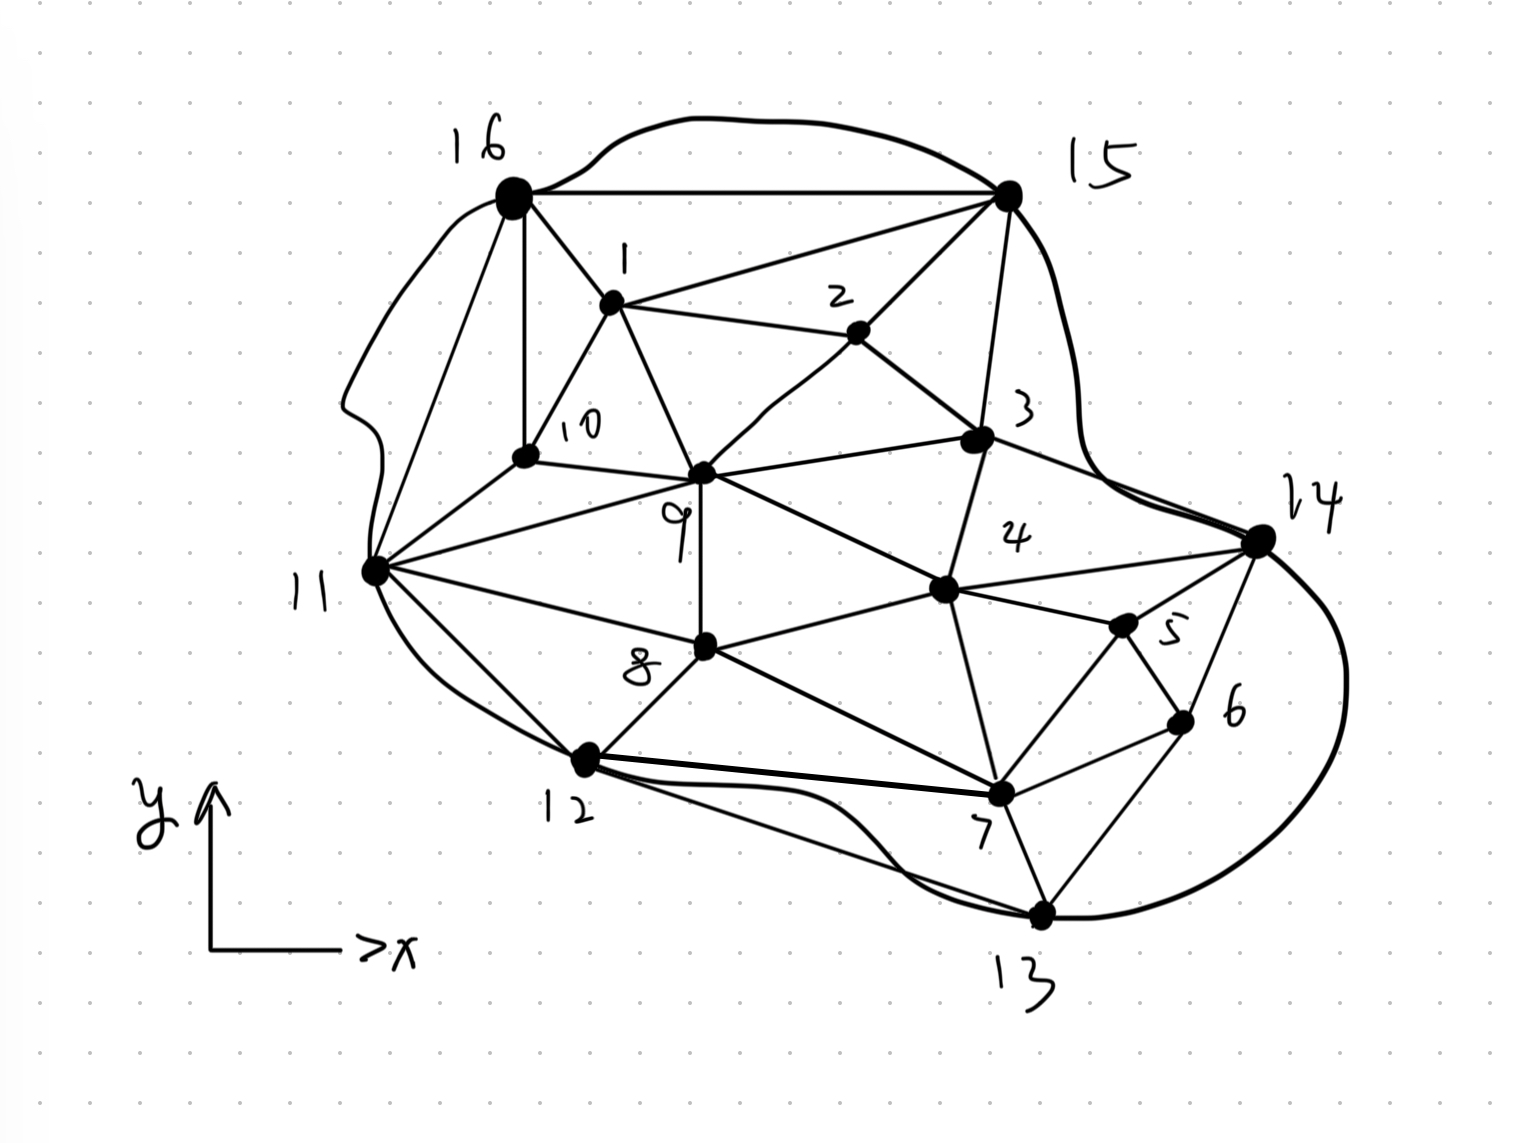
\includegraphics[width=0.5\textwidth]{figure/FIG_POSSION_2D_10_NODES.jpg}
  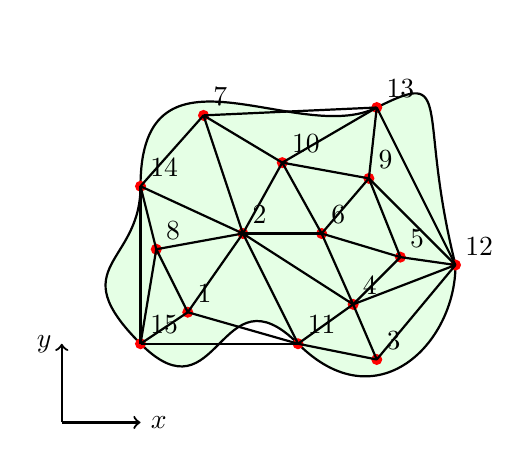
\begin{tikzpicture}
    \foreach \x/\y [count=\i from 1] in {
      1.6/1.4, %1
      2.3/2.4, %2
      4/0.8,  %3
      3.7/1.5, %4
      4.3/2.1, %5
      3.3/2.4, %6
      1.8/3.9, %7
      1.2/2.2, %8
      3.9/3.1, %9
      2.8/3.3, %10
      3/1, %11
      5/2, %12
      4/4, %13
      1/3, %14
      1/1} %15
      { 
        \coordinate (P\i) at (\x,\y);
      % \fill[red] (\x,\y) circle (3pt);
      % \node[above right] at (\x,\y) {P\i};
  }
    \draw[thick, fill=green!10] (P11) 
      .. controls (4,0)   and (5,1)   .. (P12)
      .. controls (4.5,4) and (5,4.5) .. (P13) 
      .. controls (3,3.5) and (1,5)   .. (P14)
      .. controls (1,2)   and (0,2)   .. (P15) 
      .. controls (2,0)   and (2,2)   .. (P11);
  
  \foreach \x in {1,2,3,4,5,6,7,8,9,10,11,12,13,14,15} 
  {
    \fill[red] (P\x) circle (2pt);    % 填充红色圆点
    \node[above right] at (P\x) {$\x$}; % 标记点的标签
  }

  % \node[above right] at (0,0) {$O$};
  \draw[thick, ->] (0,0) -- (1,0) node[right, right] {$x$};
  \draw[thick, ->] (0,0) -- (0,1) node[left, left] {$y$};

  \draw[thick,-] (P2) -- (P1);
  \draw[thick,-] (P2) -- (P6);
  \draw[thick,-] (P2) -- (P7);
  \draw[thick,-] (P2) -- (P10);
  \draw[thick,-] (P2) -- (P8);
  \draw[thick,-] (P2) -- (P4);

  \draw[thick,-] (P6) -- (P10);
  \draw[thick,-] (P6) -- (P9);
  \draw[thick,-] (P6) -- (P5);
  \draw[thick,-] (P6) -- (P4);

  \draw[thick,-] (P10) -- (P7);
  \draw[thick,-] (P10) -- (P9);
  \draw[thick,-] (P10) -- (P13);

  \draw[thick,-] (P9) -- (P5);
  \draw[thick,-] (P9) -- (P13);
  \draw[thick,-] (P12) -- (P13);
  \draw[thick,-] (P9) -- (P12);

  \draw[thick,-] (P5) -- (P4);
  \draw[thick,-] (P5) -- (P12);
  \draw[thick,-] (P3) -- (P12);
  \draw[thick,-] (P4) -- (P12);

  \draw[thick,-] (P4) -- (P3);
  \draw[thick,-] (P1) -- (P8);
  \draw[thick,-] (P1) -- (P15);
  \draw[thick,-] (P15) -- (P8);
  \draw[thick,-] (P15) -- (P11);
  \draw[thick,-] (P15) -- (P14);
  \draw[thick,-] (P7) -- (P14);
  \draw[thick,-] (P7) -- (P13);

  \draw[thick,-] (P14) -- (P2);
  \draw[thick,-] (P8) -- (P14);

  \draw[thick,-] (P11) -- (P3);
  \draw[thick,-] (P11) -- (P1);
  \draw[thick,-] (P11) -- (P4);
  \draw[thick,-] (P11) -- (P2);


  \end{tikzpicture}
  \caption{The Schematic Representa of of a 2D Computiational Domain and Grid. The nodes are used for the FDM by solid circles. 
  Nodes $11-15$ denote boundary nodes, while nodes $1-10$ denote internal nodes.}
  \label{FIG_POSSION_2D_10_NODES}
\end{figure}
In this case, we only need to find the value of internal nodes which $i$ is ranging from $1$ to $10$.
Next is aimming to solve this linder system \ref{EQ_POSSION_2D_10_NODES}.


\subsection{Physics Informed Neural Networks}\label{SEC:PINN}
With the explosive growth of avaliable data and computing resouces, 
recent advances in machine learning and data analytics have yieled good results across science discipline, 
including Convolutional Neural Networks (CNNs) \cite{CNN}
for image recoginition, 
Generative Pre-trained Transformer (GPT) \cite{GPT}
for natual language processing and 
Physics Informed Neural Networks (PINNs) \cite{PINN}
for handling science problems with high complexity.
PINNs is a type of machine learning model makes full use of the benefits from 
Auto-differentiation (AD) \cite{AD}
which led to the emergence of a subject called 
Matrix Calculus \cite{Matrix_Calculus}.
Considering the parametrized and nonlinear PDEs of the general form [E.q. \ref{EQ_General_PDEs}] of function $u(t,x)$
\begin{equation}\label{EQ_General_PDEs}
  u_t + \mathcal{N}\left[u;\lambda\right] = 0
\end{equation}
The $\mathcal{N}[\cdot;\lambda]$ is a nonlinear operator which parametrized by $\lambda$.
This setup includes common PDEs problems like heat equation, and black-stokz equation and others.
In this case, we setup a neural network $NN[t,x;\theta]$ which has trainable weights $\theta$ and takes 
$t$ and $x$ as inputs, outputs with the predicting value $\hat{u}(t,x)$.
In the training process, the next step is calculating the necessary derivatives of $u$ with the respect to $t$ and $x$.
The value of loss function is a combination of the metrics of how well does these predictions fit the given conditions and 
fit the natural law [Fig. \ref{FIG_Schematic_View_PINN}]. 
% \begin{figure}[htbp]
%   \centering
%   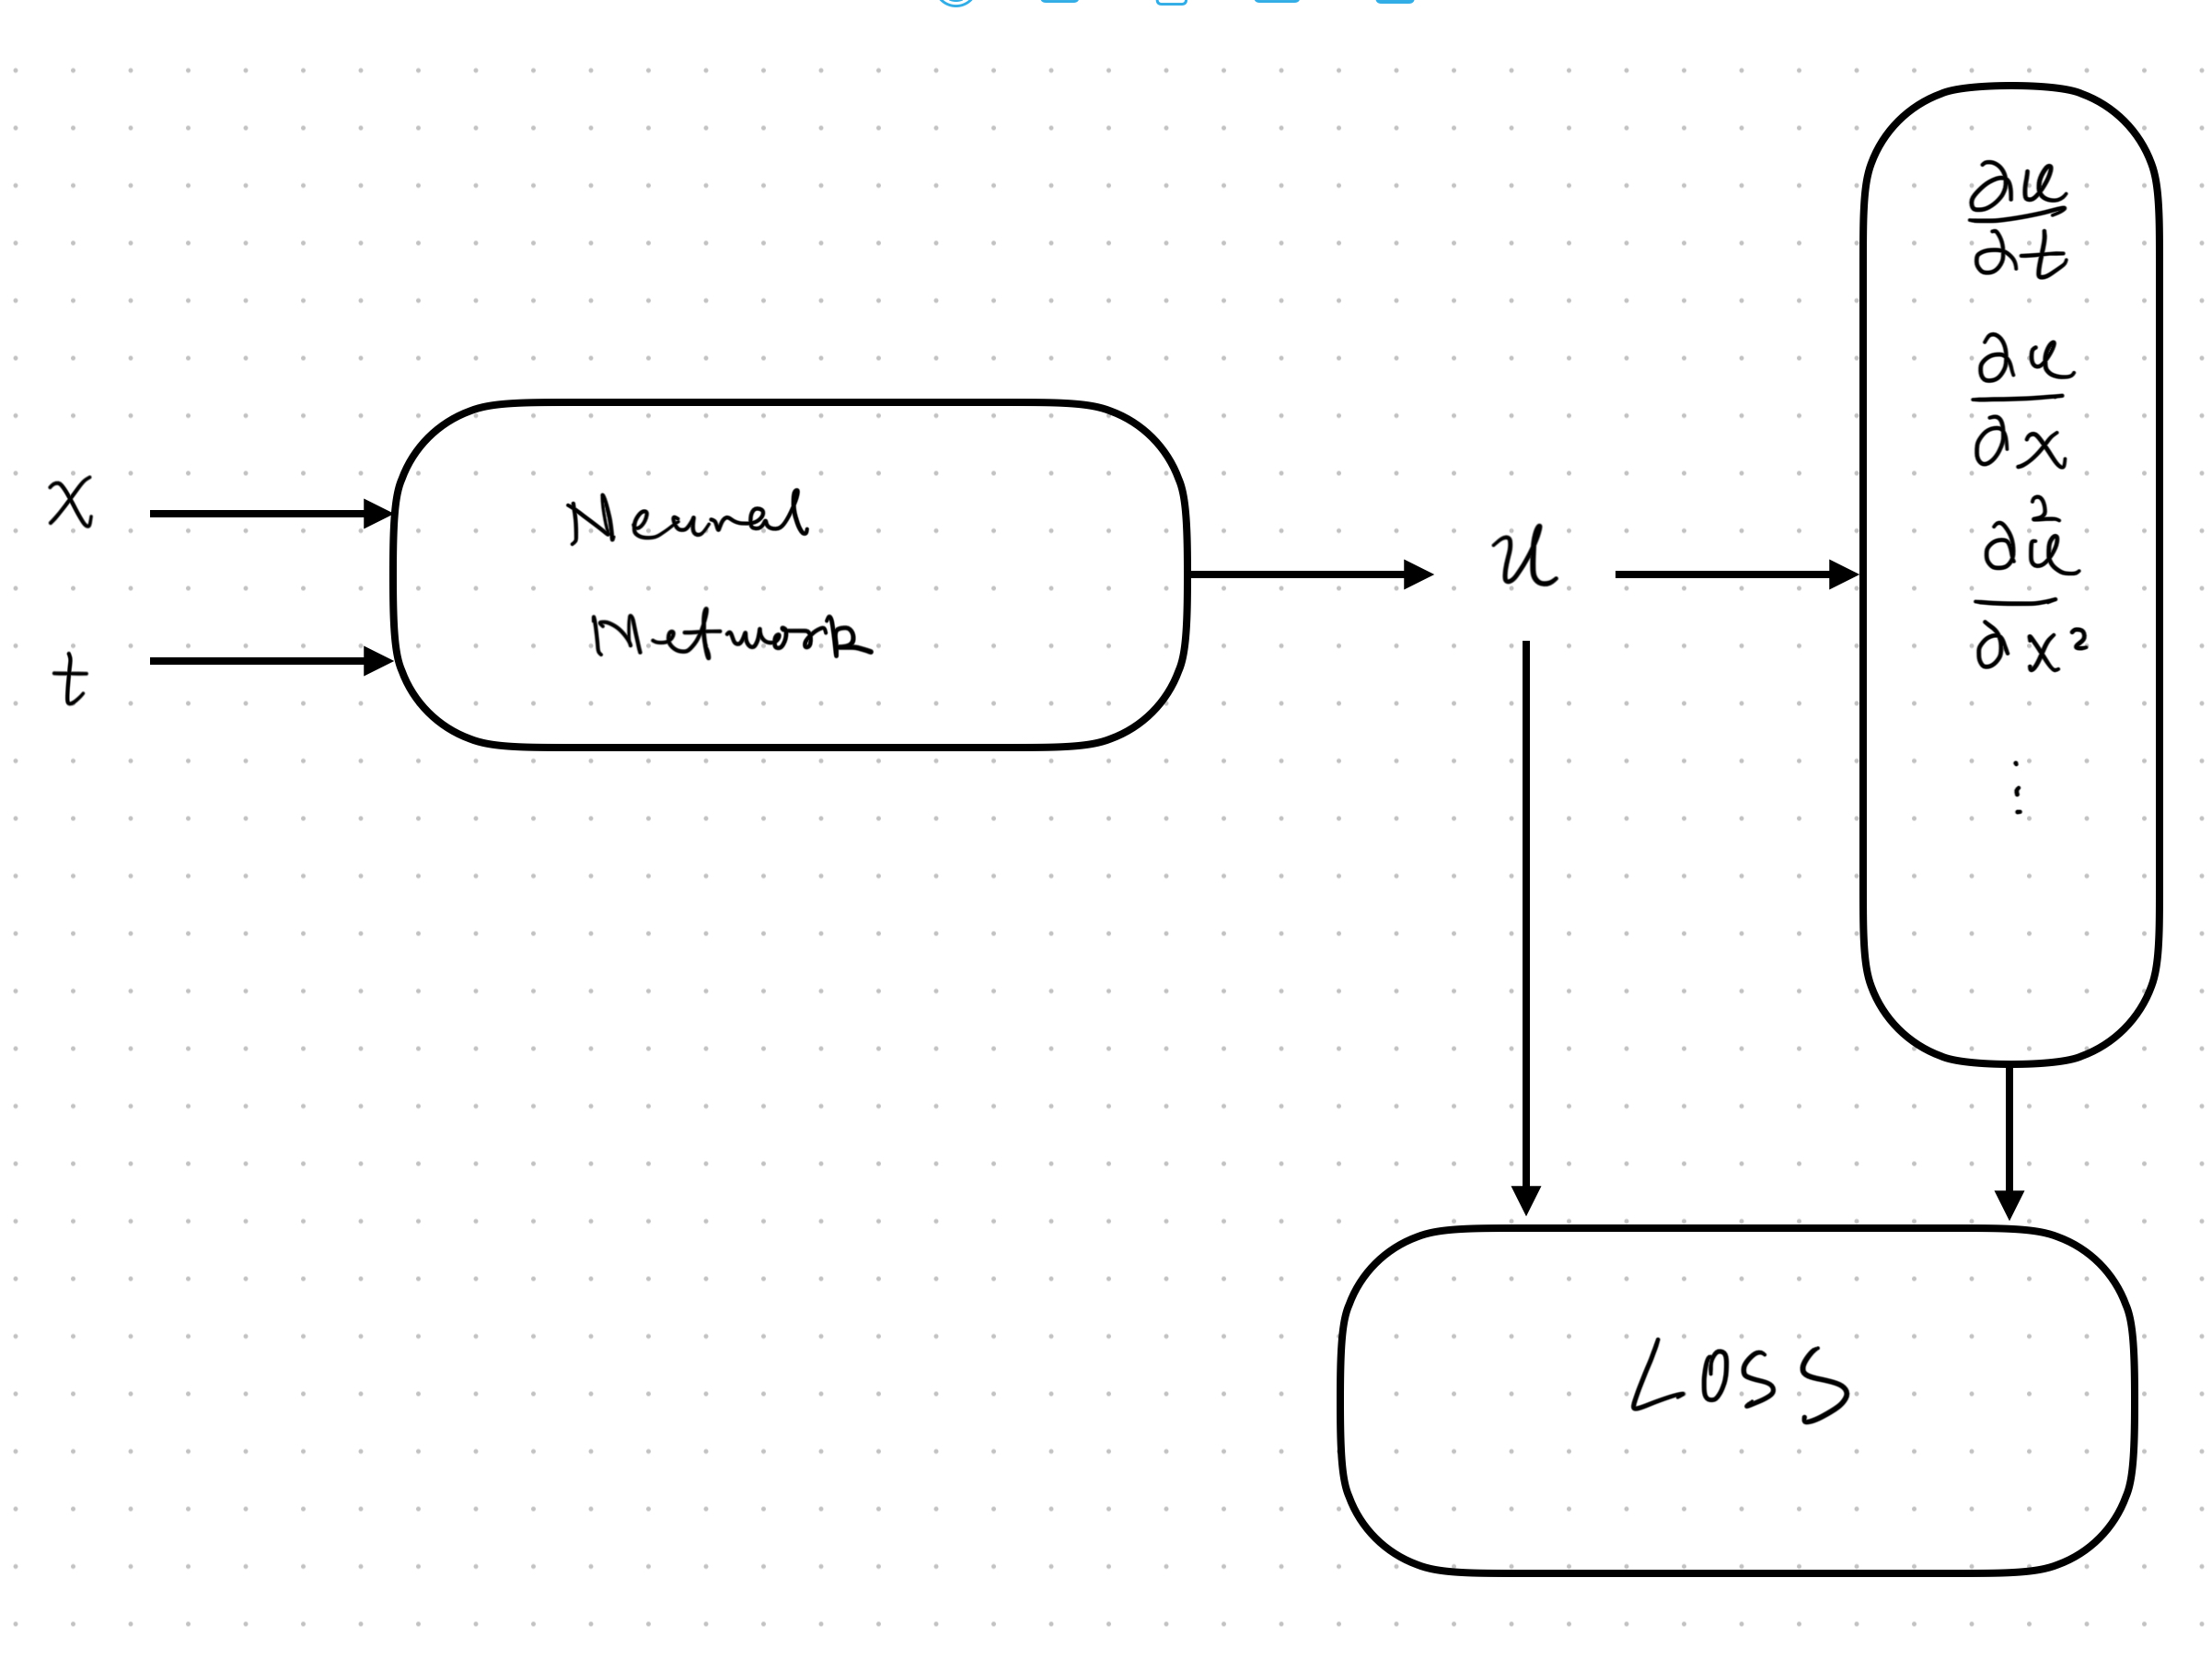
\includegraphics[width=0.5\textwidth]{figure/FIG_Schematic_View_PINN.jpg}
%   \caption{The Schematic Representa of a structure of PINN.}
%   \label{FIG_Schematic_View_PINN}
% \end{figure}


\begin{figure}[htbp]
  \centering
  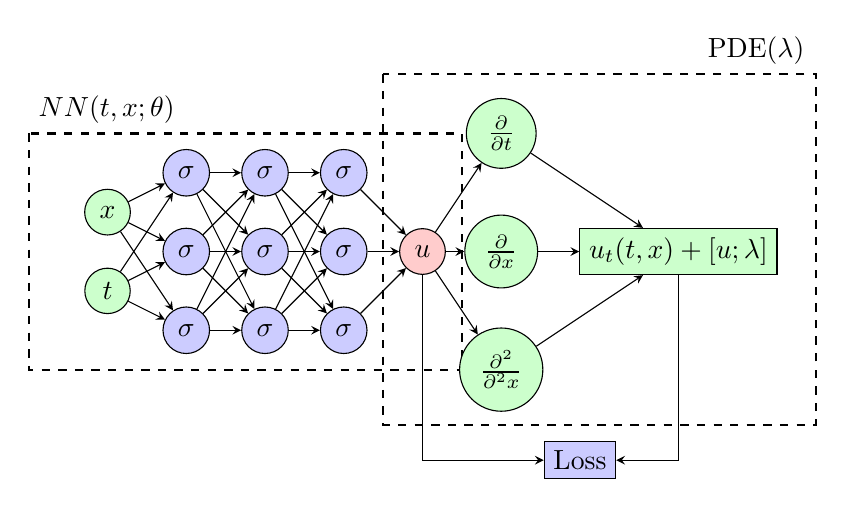
\begin{tikzpicture}[
    % Define styles
    neuron/.style={circle,draw,minimum size=.2cm},
    func/.style={rectangle,draw,minimum size=.2cm},
    PDE/.style={func, fill=green!20},
    loss/.style={func, fill=blue!20},
    input/.style={neuron, fill=green!20},
    hidden/.style={neuron, fill=blue!20},
    output/.style={neuron, fill=red!20},
    diff/.style={neuron, fill=green!20},
    arrow/.style={->,>=stealth},
    scale=0.5
  ]
    
  % \steporfull<1->{
    % Input Layer
    \draw[dashed, thick] (-2,1) rectangle (9,-5); % 前两个坐标为矩形左下角的坐标,后两个坐标为矩形右上角的坐标
    \node at (-2,1) [above right] {$NN(t,x; \theta)$}; % 文本内容为"文本",位置为方框的左上角

    \node[input] (Input0) at (0,-1) {$x$};
    \node[input] (Input) at (0,-3) {$t$};
  
    % Hidden Layer 1
    \node[hidden] (Hidden11) at (2,0) {$\sigma$};
    \node[hidden] (Hidden12) at (2,-2) {$\sigma$};
    \node[hidden] (Hidden13) at (2,-4) {$\sigma$};
  
    % Hidden Layer 2
    \node[hidden] (Hidden21) at (4,0) {$\sigma$};
    \node[hidden] (Hidden22) at (4,-2) {$\sigma$};
    \node[hidden] (Hidden23) at (4,-4) {$\sigma$};
  
    % Hidden Layer 3
    \node[hidden] (Hidden31) at (6,0) {$\sigma$};
    \node[hidden] (Hidden32) at (6,-2) {$\sigma$};
    \node[hidden] (Hidden33) at (6,-4) {$\sigma$};

    % Output Layer
    \node[output] (Output) at (8,-2) {$u$};

    % Connect neurons Input-Hidden Layer 1
    \foreach \i in {1,2,3}
        \draw[arrow] (Input) -- (Hidden1\i);
      \foreach \i in {1,2,3}
        \draw[arrow] (Input0) -- (Hidden1\i);
  
    % Connect neurons Hidden Layer 1-Hidden Layer 2
    \foreach \i in {1,2,3}
        \foreach \j in {1,2,3}
            \draw[arrow] (Hidden1\i) -- (Hidden2\j);
  
    % Connect neurons Hidden Layer 2-Hidden Layer 3
    \foreach \i in {1,2,3}
        \foreach \j in {1,2,3}
            \draw[arrow] (Hidden2\i) -- (Hidden3\j);
  
    % Connect neurons Hidden Layer 3-Output
    \foreach \i in {1,2,3}
        \draw[arrow] (Hidden3\i) -- (Output);
  % }

  % \steporfull<2->{
    \draw[dashed, thick] (7,2.5) rectangle (18,-6.4);
    \node at (15,2.5) [above right] {PDE($\lambda$)}; % 文本内容为"文本",位置为方框的左上角
    % Partial Derivatives
    \node[diff] (D1) at (10,1) {$\frac{\partial}{\partial t}$};
    \node[diff] (D2) at (10,-2) {$\frac{\partial}{\partial x}$};
    \node[diff] (D3) at (10,-5) {$\frac{\partial^2}{\partial^2 x}$};
    \node[PDE] (PDE) at (14.5,-2) {$u_t(t,x) + \varGamma \left[u; \lambda \right]$};

    \foreach \i in {1,2,3}
        \draw[arrow] (Output) -- (D\i);
    \foreach \i in {1,2,3}
        \draw[arrow] (D\i) -- (PDE);
  % }

  % \steporfull<2->{
    \node[loss] (L) at (12,-7.3) {Loss};

    \draw[arrow] (Output) |- (L);
    \draw[arrow] (PDE) |- (L);
  % }
  \end{tikzpicture}
  \caption{The Schematic Representation of a structure of PINN, a FCN with 4 layers (3 hidden layers)}
  \label{FIG_Schematic_View_PINN}
\end{figure}

\subsection{Finite Difference Time Domain Method}
As described previously in the 
section \ref{SEC:FDM}, FDM could solve the PDEs in its original form where 
Finite Element and Finite Volume Methods gained results by solving modified form such as an integral form of the governing equation.
Though the latter methods are commonly get better results or less computational hungery, 
the FDM has many descendants, 
for instance the Finite Difference Time Domain Method (FDTD) where it still finds prolific usage are computational heat equation and 
computational electromagnetics (Maxwell's equations \cite{Maxwell_equations}). 
Assuming the operator $\mathcal{N}[\cdot;\lambda]$ is set to $\nabla$ where it makes E.q. \ref{EQ_General_PDEs} become 
to heat equation \ref{EQ_HEAT_EQ_EG}.
\begin{equation}\label{EQ_HEAT_EQ_EG}
  \frac{\partial u}{\partial t} 
  - \lambda \left(
    \frac{\partial^2 u}{\partial x^2}  + \frac{\partial^2 u}{\partial y^2} 
  \right) = 0
\end{equation}
Using the key idea of FDM, assuming the step size in spatio-time space are $\Delta x$, $\Delta y$ and $\Delta t$,
we could have a series equations which have form [E.q. \ref{EQ_FDM_FDTD_EQ}].
\begin{equation}\label{EQ_FDM_FDTD_EQ}
  \frac{u^{n+1}_{i,j} - u^n_{i,j}}{\Delta t} 
  = 
  \lambda
  \left(
    \frac{
      u^n_{i+1,j} - 2u^n_{i,j} + u^n_{i-1,j}
    }{\Delta x^2}
    +
    \frac{
      u^n_{i,j+1} - 2u^n_{i,j} + u^n_{i,j+1}
    }{\Delta y^2}
  \right)
\end{equation}
when the time step size satisfies the 
Couran, Friedrichs, and Lewy condition (CFL\cite{CFL_limitation}).
We could get the strong results by iterating the equation \ref{EQ_FDM_FDTD_EQ}, or more specifically using 
equation \ref{EQ_FDM_FDTD_EQ_Iterating} to get the value $u$ of next time stamp $n+1$ on nodes $i,j$.
\begin{equation}\label{EQ_FDM_FDTD_EQ_Iterating}
  u^{n+1}_{i,j}
  = 
  u^n_{i,j} + 
    \frac{
      \lambda\Delta t
    }{\Delta x^2}\left(
      u^n_{i+1,j} - 2u^n_{i,j} + u^n_{i-1,j}
    \right)
    +
    \frac{
      \lambda\Delta t
    }{\Delta y^2}\left(
      u^n_{i,j+1} - 2u^n_{i,j} + u^n_{i,j+1}
    \right)
\end{equation}
also shown in the figure \ref{FIG:Scheme_FDTD_2D_Heat}.
\begin{figure}[htbp]
  \centering
  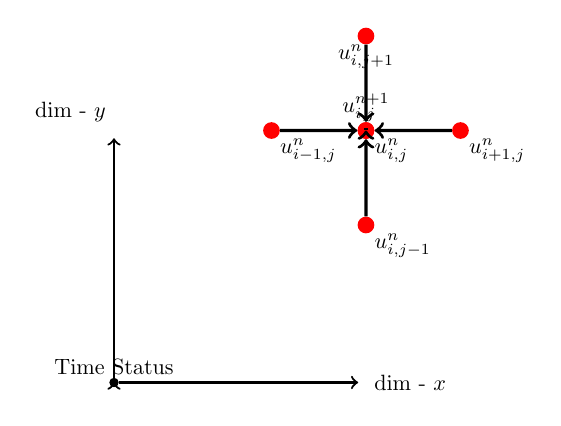
\begin{tikzpicture}[scale=0.8, transform shape]
    \def\h{10};
    \def\scale{0.8};

    \begin{scope}
      \myGlobalTransformation{0}{0};
      \graphLinesHorizontal;
      \graphLinesVertical;
    \end{scope}
    \graphThreeDnodes{0}{0};

    \begin{scope}
      \myGlobalTransformation{0}{\h};
      \graphLinesHorizontal;
      \graphLinesVertical;
    \end{scope}
    \graphThreeDnodes{0}{\h};

    \begin{scope}
      \myGlobalTransformation{0}{0};
      \node (orig) at (0,0) [circle, fill=black, scale=0.45] {};
      \node (x) at (4,0) {};
      \node (y) at (0,4) {};

      \node (this) at (4,4) [circle, fill=red, scale=\scale] {};

      \node (left) at (2.5,4) [circle, fill=red, scale=\scale] {};
      \node (back) at (4,2.5) [circle, fill=red, scale=\scale] {};
      \node (right) at (5.5,4) [circle, fill=red, scale=\scale] {};
      \node (front) at (4,5.5) [circle, fill=red, scale=\scale] {};
    \end{scope}

    \begin{scope}
      \myGlobalTransformation{0}{12};
      \node (Horig) at (0,0) {};
    \end{scope}

    \begin{scope}
      \myGlobalTransformation{0}{\h};
      \node (other) at (4,4) [circle, fill=red, scale=\scale] {};
    \end{scope}

    \draw[very thick,->] (this) node[below right] {$u^{n}_{i,j}$} -- (other) node[above] {$u^{n+1}_{i,j}$};
    \draw[very thick,->] (left) node[below right] {$u^{n}_{i-1,j}$} -- (other) node[right] {};
    \draw[very thick,->] (back) node[below right] {$u^{n}_{i,j-1}$} -- (other) node[right] {};
    \draw[very thick,->] (right) node[below right] {$u^{n}_{i+1,j}$} -- (other) node[right] {};
    \draw[very thick,->] (front) node[below] {$u^{n}_{i,j+1}$} -- (other) node[right] {};

    \draw[thick, ->] (orig) -- (Horig) node[above] {Time Status};
    \draw[thick, ->] (orig) -- (x) node[right] {dim - $x$};
    \draw[thick, ->] (orig) -- (y) node[above left]  {dim - $y$};;

  \end{tikzpicture}
  \caption{The Schematic Representation the computational spatio-temporal domain of FDTD methods.}
  \label{FIG:Scheme_FDTD_2D_Heat}
\end{figure}



\subsection{Scalability}
High performance computing which also called 
parallel computing
is solving large scale problems using Clusters, with a number of compute nodes and many CPUs.
Parallel computing is many CPUs, thousands of CPUs in most case, are simultaneously processing the data and 
producing the exceptional results, which significantly reduce the time consumption totally.
In this scenario, scaling test is a widely used to investigate the ability of hardware and programs to 
deliver more computational power when the amount of compute resources increase.

\subsubsection{Amdalh's Law and Strong Scaling}
The Amdalh's law for speedup is 
\begin{theorem}\label{THEO:Amdalh's law}
  Let $f_s$ and $f_p$ be the fraction of time spend on purely sequential tasks and that can be parallelized, then 
  the Amdalh's formula
  \cite{Amdalh'sLaw} of final speedup is
  \begin{equation}\label{EQ:Amdalh's law}
    S_N = \frac{1}{f_s + \frac{f_p}{N}}
  \end{equation}
\end{theorem}
and it states that for a fixed problem, the upper limits of speedup is restricted by the fraction of sequential parts, 
where the limits is $\lim_{N\to +\infty} S_N = 1 / f_s$, which is called the strong scaling.


\subsubsection{Gustafsson-Barsis' Law}
The Gaustafsson-Barsis' law for speedup is 
\begin{theorem}\label{THEO:GaustafssonLaw}
  Let $f_s$ and $f_p$ be the fraction of time spend on purely sequential tasks and that can be parallelized, then 
  the Gaustafsson-Barsis' formula 
                                                        \cite{GaustafssonLaw}
  of the final speedup is 
  \begin{equation}\label{EQ:GaustafssonLaw}
    S_N = f_s + Nf_p
  \end{equation}
\end{theorem}
With Gaustafsson-Barsis's law, the scaled speedup increases linearly with the number of processes, and there is no upper 
limits for the scaled speedup, which is called weak scaling.

The weak scaling tests of an high performance program runing on cluster is necessary for researching the inner relationships 
between the number of CPUs and the scale of problems.
In order to get better weak scaling performance, the fraction of synchronization among processes and the cost of communications 
plays a minor role when the number of resources increase. 
In the meanwhile, unlike the strong scaling test, the iterations takes for converging on different problem sizes are various as well.
Thus, the weak scaling is more effective if it only consider the scaling for single iteration, where the speedup 
on $N$ CPUs has formula follows
\begin{equation}
  S_N = N\frac{T_1C_N}{C_1T_N} 
\end{equation}
where $T_N$ and $C_N$ denote with the time and epochs that the solver takes for converging on $N$ CPUs.

\section{Problem Setups}
Due to the inherent limitations of current computing systems, 
obtaining sufficiently precise solutions is both computationally expensive and time-consuming. 
These challenges arise from the constraints imposed by the clock speed of computing units, 
as described by 
Moore's Law \cite{Moore_Law}, 
as well as the relatively low communication speeds between these units. 
While modern numerical methods have advanced to a level where they can produce 
satisfactory results within acceptable time frames across many research domains, 
the increasing scale of problems we aim to solve has driven the search for more 
cost-effective approaches. This has led to a growing interest in neural networks as a promising alternative.

In this project, I aim to evaluate the performance of the Finite-Difference Time-Domain (FDTD) 
method and the Physics-Informed Neural Network (PINN) model within parallelized computing 
environments by find the steady-state solution of PDEs.
These two methodologies broadly represent the current approaches to 
handling PDEs, specifically 
CPU-based parallelization and GPU-based parallelization.

\subsection{General Form}\label{SEC_General_Form}
Starting with the general form of the PDEs, rather than the specific euqations, is because 
different equations give perform differently on the same compute system.
To this end, consider the previously discussed form of PDEs shown in 
equation \ref{EQ_General_PDEs} which parametrized by number $\lambda$ and an operator $\mathcal{N}[\cdot; \lambda]$.
Moreover, we assume the variable $x$ is a 2D or 3D spatio vector which is written in 
$\vec{x} \in \mathbb{R}^d$, $d = 2, 3$.
\begin{align}\label{EQ_General_Form_PDE}
  &\frac{\partial u}{\partial t}\left(t,\vec{x}\right) + \mathcal{N}\left[u(t,\vec{x});\lambda\right] = 0, &\vec{x}\in\Omega, &t\in[0, +\infty) \nonumber\\
  &u\left(0,\vec{x}\right) = \varphi (\vec{x}), &\vec{x}\in\Omega & \\
  &u\left(t,\vec{x}\right) = g (t,\vec{x}),     &\vec{x}\in \overline{\Omega}, &t\in[0, +\infty) \nonumber
\end{align}
The domain of this PDE system is considered between $0$ and $1$, where is denoted with $\Omega = [0, 1]^d$, $d = 2,3$.
To these setups, we have the general form of the PDEs we are going to investigated, shown in equations \ref{EQ_General_Form_PDE}
The boundary condition shown in E.q. \ref{EQ_General_Form_PDE} is Dirichlet Condition known as first type boundary condition, where as the 
second type boundary condition (Von Neumman) [E.q. \ref{EQ_Von_Neumman_BC}] gives the other form of $u(t,\vec{x})$ at the boundary $\overline{\Omega}$.
\begin{equation}\label{EQ_Von_Neumman_BC}
  \frac{\partial u}{\partial \vec{x}} = g(t, \vec{x}),\:\: \vec{x}\in \overline{\Omega}, \:\:t\in[0, +\infty)
\end{equation}

\subsection{Specific Form}\label{SEC:Specific_Form}
With general form proposed in section \ref{SEC_General_Form}[E.q. \ref{EQ_General_Form_PDE}],
I specify a particular form of this heat problem to help us to have better understand the quality of our 
solutions and programs.
In $2$ dimension space, the domain $\Omega = \left[ 0, 1\right] ^2 \in \mathbb{R}^2$ and its boundary
denoted with $\overline{\Omega}$, the initial condition $\varphi(x,y) = 0$.
such problem has the certain form below
\begin{align}\label{EQ:Heat2D}
  &\frac{\partial u}{\partial t} = \alpha \left(
    \frac{\partial u^2}{\partial^2 x}
    +
    \frac{\partial u^2}{\partial^2 y}
  \right) &(x,y) \in \Omega, \: t \in \left[0, +\infty\right)  \nonumber\\
  &u(0,x,y)  = \varphi(x,y) = 0 &(x,y) \in \Omega\\
  &u(t,x,y)
   = g(x,y)
   = \begin{cases}
    y, \:\: x=0, y\in\left(0,1\right)\\
    1, \:\: x=1, y\in\left(0,1\right)\\
    x, \:\: y=0, x\in\left(0,1\right)\\
    1, \:\: y =1, x\in\left(0,1\right)
  \end{cases}
  &t \in \left[0, +\infty\right) \nonumber
\end{align}
With given format, and $\alpha = 1$, we have the analytical solution of this equations, where is 
\begin{equation}\label{EQ_SOLUTION_2D}
  u(t,x,y) = x + y - xy, \:\:(x,y) \in \Omega,\: t \in \left[0, +\infty\right)
\end{equation}
In 3 dimension space, similarly, with identical initial condition set up to $0$, coefficient $\alpha = 1$,
the boundaries are 
\begin{equation}
  u(t,x,y,z) = g(x,y,z) = 
  \begin{cases}
    y+z -2yz        , \:\: &x=0,\\
    1 - y - z + 2yz , \:\: &x=1,\\
    x+z - 2xz       , \:\: &y=0,\\
    1 - x - z + 2xz , \:\: &y =1,\\
    x+y - 2xy       , \:\: &z=0,\\
    1 - x - y + 2xy , \:\: &z=1
  \end{cases}
  \:\:, t \in \left[0, +\infty\right)
\end{equation}
In such case, the analytical solution has for form below 
\begin{equation}
  u(t,x,y,z) = x + y + z - 2xy - 2xz - 2yz + 4xyz, \:\:(x,y,z) \in \Omega,\: t \in \left[0, +\infty\right)
\end{equation}


\subsection{Discretization}
To begin with discretizing the objects or regions we intend to 
evaluate via matrices, we consider a straightforward approach: 
using the coordinates in $d=2,3$ dimensional spaces and the function 
values at those points to simplify the objects. 
This naive approach works well for investigating objects with regular shapes, such as a cube.

For the FDTD (Finite-Difference Time-Domain) method, we use a finely 
generated $d$-cube with shape $\left\{n_i\right\}_i^{d}$. Including 
the boundary conditions, the cube has $\prod_i (n_i+2)$ nodes. 
It requires $4\prod_i (n_i+2)$ bytes for float32 or $8\prod_i (n_i+2)$ bytes 
for float64 to store in memory. 
With this setup, for equally spaced nodes, we have:
\begin{equation}
  \Delta x_i = \frac{1}{n_i-1}
\end{equation}

Unlike the previously generated regular grid of 
points with dimensions $n_xn_yn_z$, 
another strategy is to randomly generate the same number of points based on the same known conditions, 
covering both the central part and the boundary. 
In this scenario, 
shown in figure, 
there are $n_x n_yn_z$ central points, 
with function values set according to the boundary conditions, 
and $2 \times(n_xn_y + n_yn_z + n_zn_x)$ boundary points to be solved. 
This set of points can be used for training a PINN model.

% 不同于之前生成规则的nx * ny * nz的点阵,另一种策略是对于与先前同样的已知条件随机生成同样数量的点,用于中心的部分以及边界部分。
% 这种情况下一共有nx * ny * nz个中心部分,根据边界条件设置函数值,以及(nx * ny + ny * nz + nz * nx)*2个边界点,需要求解的部分。
% 这种方式生成的点集用于训练PINN模型。
\begin{figure}[htbp]
  \centering
  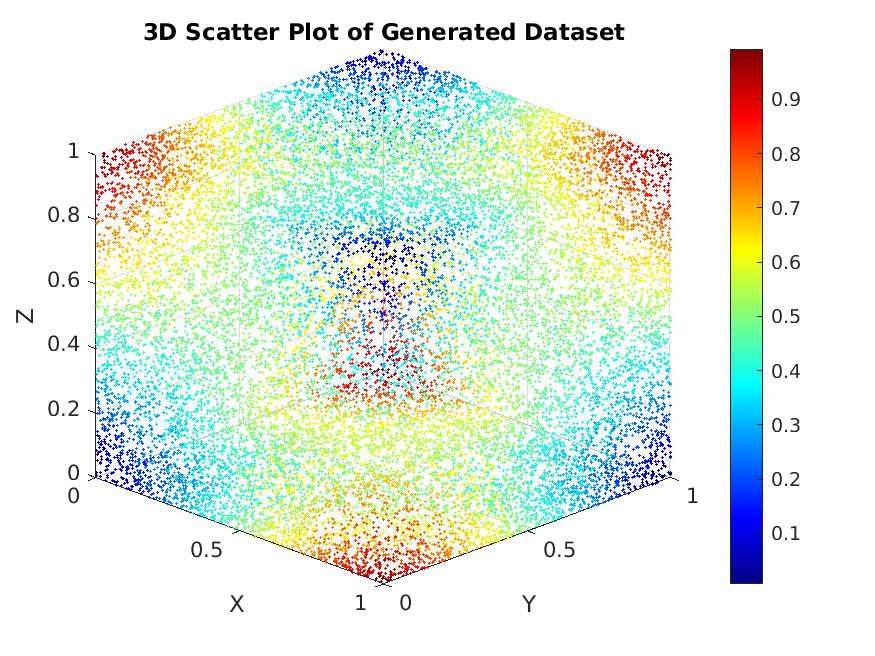
\includegraphics[width=0.5\textwidth]{figure/FIG_main2_dataset.png}
  \caption{Randomly general dataset for 3D PINN model training.}
  \label{FIG_Topology_Callan}
\end{figure}

% \begin{figure}[htbp]
%   \centering
  
%   \caption{Figure Shows the FDM idea, If NEED}
%   \label{<label>}
% \end{figure}


\subsection{Accuracy}
When we tried to represent numbers using arithmetic in binary, decimal or hexadecimal, truncation always affects the precision of every number, 
or so called as 
round-off-error.

\subsubsection{Round-off Error}
In IEEE-754 \cite{IEEE_754} standards, a $32$-bit floating pointer number, single precision, obligatorily represented with $23$-bit mantissa, 
$8$-bit exponent and $1$-bit for sign. 
Where as $64$-bit floating number, double precision, also ubiquitous used, which has $11$-bit exponent and $52$-bit mantissa.
After almost three decades development, not only single and double precisions (float32, float64) are ubiquitously in use, 
also more formats such as fp4, fp8, and fp16 etc. Both of them follows the simple form of exponent $k$, sign $n$ and mantissa $N$. 
\cite{IEEE_754_p2_eq1}
\begin{equation*}
  2^{k+1-N}n
\end{equation*}
Round-off errors are a manifestation of the fact that on a digital computer, which is unavoidable in numerical computations.
In such case, the precision of the number depends on how many bytes are used to store single number. 
For instance, a float32 number provides $2^{-23} \approx 1.2\times10^{-7}$, and a double precision number gives $2^{-53} \approx 2.2\times10^{-16}$, 
such number is called machine $\epsilon$ which is the smallest number the machine can represent with given format.

In numerical methods I investigated, the FDTDs are conventionally using double precision number so that the programs can treat extreamly large and small 
numbers simultaneously in the same computation, without worring about the round-off errors.
However, as mentioned, fp32 and fp16 are also popular use in scientific computing, especially in machine learning training process. 
While the lasted training GPUs are integrated compute accelarate unit for low precision floating numbers. \cite{NVIDIA_HB200_PAPER}.

\subsubsection{Floating-point Arithmetic}
The other type loss comes from the arithmetic operations on two numbers $x$, $y$. 
The standard model holds that 
\begin{equation}
  fl(x \:\text{op}\: y) = (x \: \text{op} \: y) (1+\delta), \:\:\: \left|\delta\right| < \epsilon
\end{equation}
where the op stands for the four elementary operations: $+, -, \times, /$. \cite{Germund,NMSC,V1,P112}.


\subsection{Computiational Topology}
The computational topology is critically important when we are programming parallel PDEs solver softwares.
Put the strongly speed-dependent data into the slow memory could make entire program slower.

\paragraph{Callan}
The cluster we are using for this project is \texttt{Callan} \cite{Callan_TCD} which has 
$2$ CPUs per compute node, and each CPU has $32$ cores with single thread. 
The Non-Uniform Memory Access (NUMA) nodes are layout as following 
\begin{figure}[htbp]
  \centering
  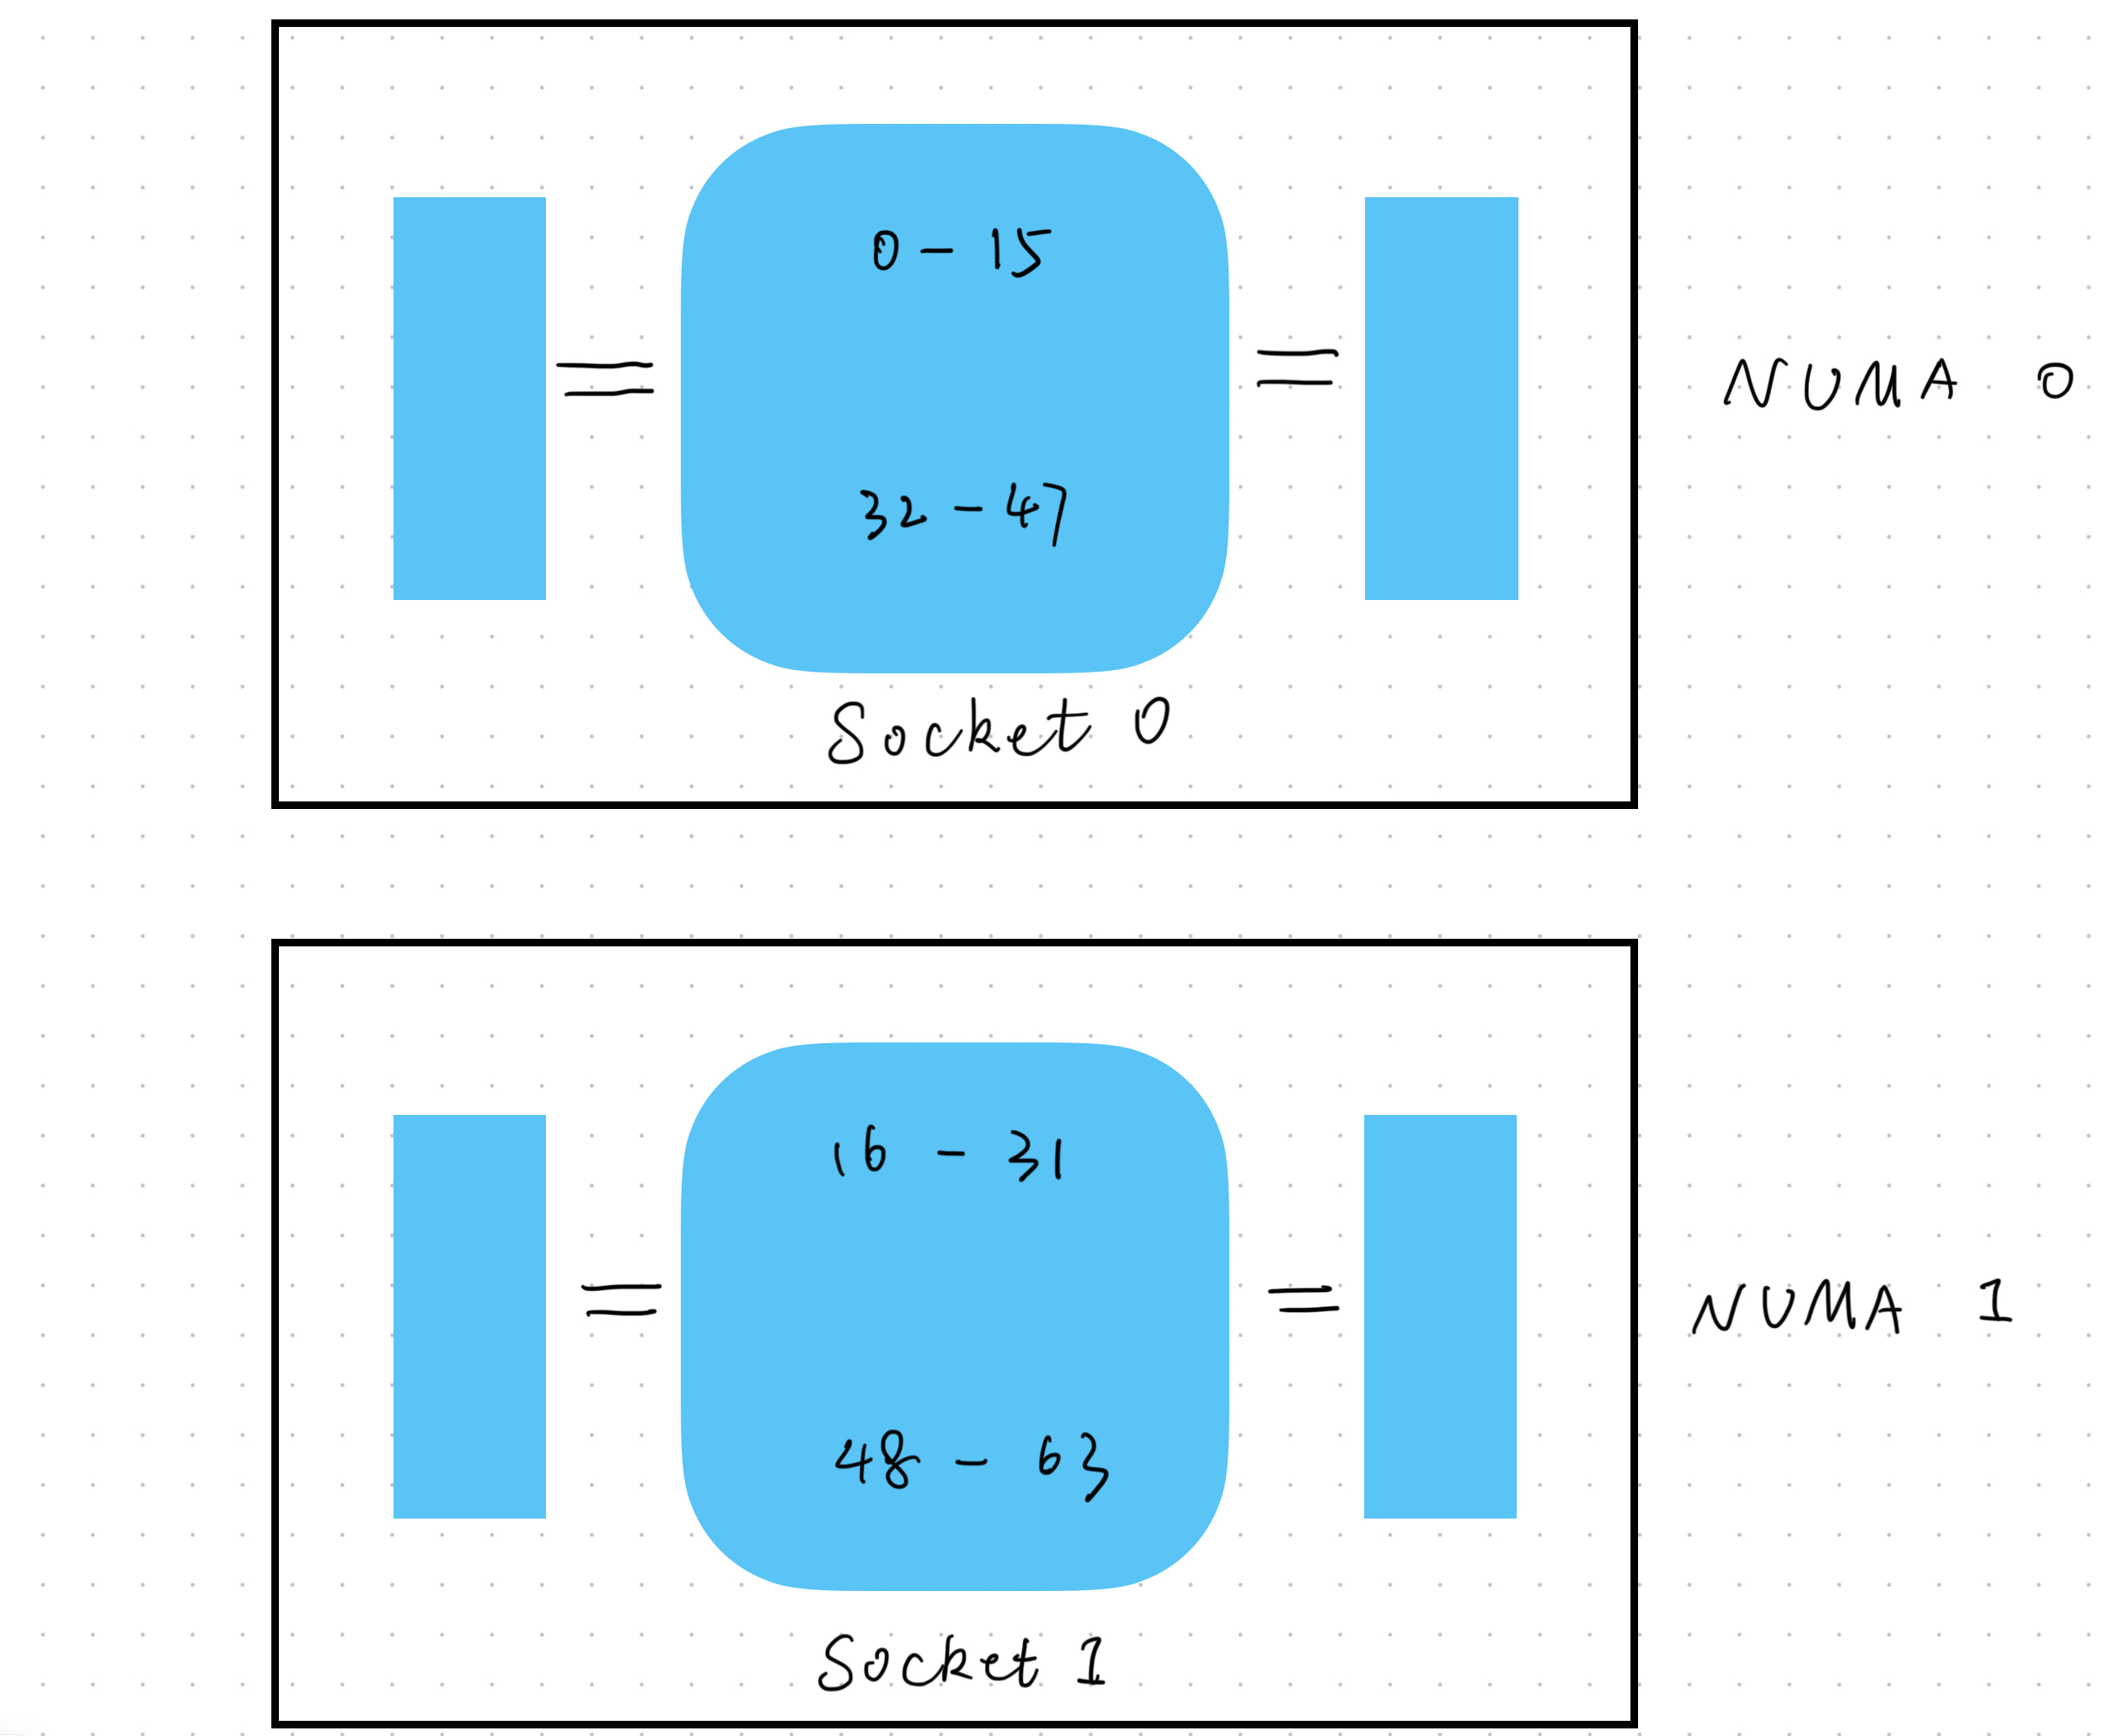
\includegraphics[width=0.5\textwidth]{figure/FIG_Topology_Callan.jpg}
  \caption{NUMA topology of single node on Callan}
  \label{FIG_Topology_Callan}
\end{figure}
Accessing the other NUMA node's memory reduces the bandwidth and also the latency,
though the bandwidth is commonly high enough, the latency can increase by 
$~30\%$ to $~400\%$ \cite{NUMA_Latency_TCD}. 
This latency becomes dangerous when writing shared memory parallel programs.

\section{Methedology}
\subsection{General Setups}
Initially, we need to determine the data types to be used and define macros for 
assertions and helper functions to ensure that the program can detect common bugs 
and report their locations. 
These features can also be disabled in the release version for performance optimization. 
Such details are defined in the \texttt{assert.hpp}, \texttt{helper.hpp}, 
and other related header files located in the subfolder.

\subsection{Template Multi-dimension Matrix Detail Design}
The FDTD method is a type of FDM. 
The main idea behind FDM is briefly outlined in Section \ref{SEC:FDM}. 
The challenge lies in implementing it in a computer system to ensure it runs both correctly and efficiently.
Also, the data types I am using for storing sizes are unit32\_t and unit64\_t while I used them 
as Dworld and Qworld respectively, also are defined as size\_type and super\_size\_type in \_\_detail namespace.

\subsubsection{Performance Balancing}
\paragraph{Template Class}
Instead of doing this by using hierarchy in C++, which will cause the memory of object becomes complicated and unpredictable,
and leading to scattered data members between base and derived class objects.
This scattering can increase the cache misses which accessing these members, as the data might not be contiguous in memory.
Also, with deep inheritance hierarchies, program has higher change to occur diamond problems, since it increases the code complexity.
In detail, the diamond problem leads the duplicate inheritance and ambiguity in the method resolution, which will drop performance down again.
Although, it is solvable by using \texttt{virtual} inheritance, but again, it increase the complexity.

In such case, I chose to use template class to design the matrix object, which implement compile-time polymorphism as opposed runtime polymorphism
provided by inheritance and virtual functions. 
With such template design, the compiler makes the decisions about which function or class instantiate is made at compile time, eliminating 
the need for \texttt{vtable}s and indirect function calls, which leads to more efficient code. 

\paragraph{Memory Management}
Rather than using the standard library's (STL) vector module, 
which can be slower due to the overhead of row pointers, 
I opted to build the Matrix object using a unique pointer 
(
  \texttt{std::unique\_ptr}
), which includes only basic features such as reset, swap, and most importantly, 
a destructor that automatically deletes pointers. 
This approach enhances the safety of memory management in our programs.
Additionally, from a safety perspective, 
given that I implemented many features within the matrix object, 
I followed standard library conventions for naming. 
This includes using the \texttt{\_\_detail} namespace within namespace \texttt{multi\_array} to 
hide objects and features that are not intended for direct use by the end user.

\subsubsection{Template Object Design of Matrix Shape}

\paragraph{Strides} 
Besides that, in the multidimensional cases, the size in each dimension is not enough for accessing 
variables, this is where we need the \texttt{strides} member variable, which stores the 
number of element the operator needs to skip in each dimension.
The \texttt{\_\_multi\_array\_shape} object is encapsulated within 
the \texttt{\_\_detail} namespace and serves as a member variable of the later template object for the multi-dimensional matrix. 
This object includes a member variable defined using the STL vector, as the shape object primarily stores the sizes for each dimension, 
which typically requires only a small amount of space. 
Additionally, this object provides member functions to access the size of a given dimension. 
\begin{algorithm}
  \caption{Stride implementation}
  \begin{algorithmic}[1]
    \STATE \texttt{dims}    \hfill \# STL vector, stores the matrix's size in each dimension.
    \STATE \texttt{strides} \hfill \# STL vector, has the same size with dims.
    \STATE n = dims.size()  \hfill \# Store the dimension of matrix.
    \STATE strides[d-1] = 1; \hfill \# Stride is 1 in the first dimension.
    \FOR{ d = n - 1; d > 0; --d }     
      \STATE strides[d-1] = strides[d] * dims[d] \hfill \# Determine stride in the latter dimension.
    \ENDFOR
    \RETURN \texttt{strides}
  \end{algorithmic}
\end{algorithm}


\paragraph{Performace Balancing}
In certain scenarios, 
we only require the shape information of a matrix without needing to access the entire matrix object. 
Accessing the shape information through well-defined operators is a more efficient way to 
handle multidimensional matrices. 
This is particularly crucial in parallel programming, where understanding 
the shape of a matrix is of critical importance. 
Sometimes, a process may need to know the shape of matrices stored on other processes. 
In such cases, using this matrix object as a local variable within functions increases the 
likelihood that the compiler will store it in a register, 
which is generally faster than using heap or stack memory.
In addition, it includes check and cast functions that allow the user to verify if the template data type \texttt{\_\_T} is signed using \texttt{constexpr}. 
The \texttt{constexpr} keyword ensures that this check occurs at compile time, and if the data type is not legal, 
the program will assert and provide a message indicating that the indexing value must be a non-negative number. 


\subsubsection{Template of Multi-dimensional Matrix Implementation}
The Matrix in this project is designed to support various data types in C++. 
Consequently, the matrix is implemented as a template class with several essential features, template 
variable \texttt{\_\_T} and \texttt{\_\_NumD}, for the value data type and number of dimension, 
also including iterators, swap functionality, fill operations, and support for the IO stream operator \texttt{<<}. 
To facilitate this, the \texttt{\_\_array\_shape} object is used to explicitly manage and access the array's shape information. 


\paragraph{Operator \texttt{()}}
The hard part of this object designed is the support template number of dimension, whereas the dimension 
is integer not less than $1$,
the operator of access element is designed by following algorithm
\begin{algorithm}
  \caption{Operator \texttt{(Ext ... exts)} of template matrices object \texttt{\_\_detail::\_\_array}}
  \begin{algorithmic}[1]
    \STATE \texttt{\_\_NumD}, \texttt{\_\_T};                   \hfill \# Template variables: dimension, data type.
    \STATE \texttt{FINAL\_PROJECT\_ASSERT\_MSE}                 \hfill \# Number of Arguments must Match the dimension.
    \STATE \texttt{index} = 0, \texttt{i} = 1                \hfill \# Initialize variables in advance.
    \STATE \texttt{indices[] = \_\_shape.check\_and\_cast(ext)}          \hfill \# The indexes number must none-negative number.
    \FOR{i < \texttt{\_\_NumD}; ++i}
      \STATE \texttt{index += indices[i] * \_\_shape.strides[i]} 
    \ENDFOR
    \STATE \texttt{FINAL\_PROJECT\_ASSERT\_MSE}           \hfill \# Boundary checking.
    \RETURN \texttt{\_\_data[index]}
  \end{algorithmic}
\end{algorithm}

\paragraph{Overload operator \texttt{<<}}
In order to print the multi-dimension array with operator \texttt{<<}, I designed a recursive helper function
to print the matrix on given dimension. Thus we could call the function on the first dimension, and it will 
recursively print all dimensions.
\begin{algorithm}
  \caption{Recursive Function to Print Multi-Dimensional Array}
  \begin{algorithmic}[1]
    \STATE \texttt{current\_dim}, \texttt{offset};               \hfill \# Parameters: current dimension, offset.
    \STATE \texttt{Dims} \texttt{\_\_Dims};                       \hfill \# Template variable: number of dimensions.
    \IF{\texttt{current\_dim == \_\_Dims - 1}}
      \STATE \texttt{os << "|"}                                   \hfill \# Start printing last dimension.
      \FOR{$i$ \texttt{ from 0 to arr.\_\_shape[current\_dim] - 1}}
        \STATE \texttt{os << std::fixed << std::setprecision(5) << std::setw(9) << arr.\_\_data[offset + i];} \hfill \# Print array elements with formatting.
      \ENDFOR
      \STATE \texttt{os << " |\textbackslash n";}                  \hfill \# End of current row in the last dimension.
    \ELSE
      \FOR{$i$ \texttt{ from 0 to arr.\_\_shape[current\_dim] - 1}}
        \STATE \texttt{next\_offset = offset;}                      \hfill \# Initialize next offset.
        \FOR{$j$ \texttt{ from current\_dim + 1 to \_\_Dims - 1}}
          \STATE \texttt{next\_offset *= arr.\_\_shape[j];}          \hfill \# Update next offset based on shape.
        \ENDFOR
        \STATE \texttt{next\_offset += i * arr.\_\_shape[current\_dim + 1];} \hfill \# Finalize next offset for recursion.
        \STATE \texttt{self(self, arr, current\_dim + 1, next\_offset);} \hfill \# Recursive call to print next dimension.
      \ENDFOR
      \STATE \texttt{os << "\textbackslash n";}                     \hfill \# Print a newline after each dimension.
    \ENDIF
  \end{algorithmic}
\end{algorithm}



\subsection{Template Multi-dimension Matrix Interface Design}
With contiguity of safety, this object of multi-dimension array is accessible to users without 
direct visit to the memory space where store values of matrix.

\subsubsection{Resource Acquisition Is Initialization (RAII)}\label{SEC:RAII}
This private object has only a member variable, a unique pointer to the template \texttt{\_\_array}, 
and other member function provide necessary features to operating on it.
Smart pointers acquire resources in their constructor and automatically release them in their destructor, 
which is the essence of RAII. 
By releasing resources in the destructor, smart pointers help prevent resource leaks.
When an exception occurs, smart pointers automatically release resources, preventing resource leaks,
thus it enhanced the safety level of using resources, reduce the potential memory leak problems.


\subsubsection{Template Multi-dimension IO for writing to/reading from file}
Initially, the multi-dimension matrix has variables shape, 
and values which given dimension and size in each dimension.
This template design end up with these variable can be stored in given data types also leads with lower 
portability.
To avoid such problems and from other point of views, I chose to store the matrices in binary format, 
rather than other type files.
There are couple benefits of doing so,
\begin{enumerate}
  \item 	Compatibility and Portability: The format of binary files is relatively 
  stable and can be easily used in different programming environments or applications. 
  Unlike \texttt{.txt} files, \texttt{.mat} files those has less compatibility across different platforms.
  \item I/O Performance: Binary files can perform block-level I/O operations directly 
  without needing to parse text formats or convert data types. 
  This usually makes reading and writing binary files much faster than \texttt{.txt} files, 
  especially when dealing with large-scale multidimensional matrix data.
  \item Support MPI IO: Binary files support the MPI IO, which provides a significant reduction in the 
  cost of communication, when storing and reading the large scale matrices. 
\end{enumerate}
However, the IO does not play a critical role in effects performance of FDTD algorithms, if and only if 
we need to store or load the data during evolving the arrays.

\subsection{MPI Parallel Environment Design Scheme}
\subsubsection{MPI Setups}
\paragraph{Environment}
Similar to how \texttt{malloc} in C and \texttt{new} in C++ require manual memory management, 
the MPI environment also necessitates explicit initialization and finalization. 
However, unlike the efficient implementation of smart pointers in the STL, 
Boost.MPI\cite{BOOST_MPI}
-a high-level parallelism library—
may not be the optimal choice for high-performance programs. 
Therefore, I chose to design a custom MPI environment that encapsulates the necessary features specific to this project.

The \texttt{mpi} namespace, a sub-namespace of \texttt{final\_project}, provides the \texttt{environment} class. 
This class integrates MPI initialization using the constructor, which invokes \texttt{MPI\_Init\_thread},
provides multi-threading shared memory parallelism in MPI, 
and MPI finalization through the destructor, which calls \texttt{MPI\_Finalize}.

It also offers direct access to the rank and the number of processors within the MPI communicator.
Furthermore, I have explicitly deleted the copy and move assignment operators to enhance safety. 
This design decision aligns with the RAII principle, 
ensuring that MPI environment resources are automatically managed, thereby preventing leaking and 
using-uninitialized problems.

\paragraph{Types and Assertions} 
Aligned meta-programming with polymorphism principles, 
I designed a template function to retrieve the corresponding MPI basic data types, 
leveraging the fundamental data types I defined as traits at the outset.
Moreover, I provides some MPI macros in assert file, 
these macros provide a unified interface for dealing with MPI-related errors,
ensuring that MPI errors are handling consistently, safely. 

\subsubsection{MPI Topology (\texttt{Cartesian})}
The namespace \texttt{topology} is a sub-namespace of \texttt{mpi}, 
the template Cartesian structure is the mainly used object in following 
problems.
To optimize memory usage, this object maintains only essential multi-dimension matrices' global and local shape member variables.
It also contains a MPI Communicator and MPI value data type, halo data type along with the neighbors' rank in the source and dest sites.
To ensure the MPI security, the copy and move constructors as well as assignment operators are manually removed.
Additionally, the destructor is customized for properly release halo data type and Cartesian communicator. 


\paragraph{Determine the local matrix's localtion}
Evenly distributing tasks across processes is of critical importance.
To address this, I designed an algorithm to divide an integer $N$ evenly to $n$ clients, where I could put it in use in 
many cases.
Rather than implementing a standalone function, I chose to implement a lambda function, which is a feature in C++ that do not significantly 
impact the performance.
It allows me to design a small function which is not frequently use or play a key role in performance.
\begin{algorithm}
  \caption{Lambda Function (decomposition): Split tasks evenly to $n$ processes evenly}
  \begin{algorithmic}[1]
    \STATE \texttt{n, rank} \hfill \# const Integers, total number and current rank of Processor.
    \STATE \texttt{N} \hfill \# constant Integer, Problem size.
    \STATE \texttt{s, e} \hfill \# Integer, start, end indexes.
    \STATE \texttt{n\_loc = n / N} \hfill \# Divide the problem evenly.
    \STATE \texttt{remain = n \% N} \hfill \# Get the remaining tasks.
    \STATE \texttt{s = rank * n\_loc + 1} \hfill \# Calculate the start indexes.
    \IF{\texttt{rank < remain}}      
      \STATE \texttt{s += rank}      \hfill \# Give a task to process the rank is smaller than remain.
      \STATE \texttt{++n\_loc}       \hfill \# Update local number of tasks.
    \ELSE 
      \STATE \texttt{s += remain}   \hfill \# Add the remain to start index, after split remains.
    \ENDIF
    \STATE \texttt{e = s + n\_loc + 1}  \hfill \# Get the ending indexes
    \IF{\texttt{e > n} \OR \texttt{rank == N - 1}} 
      \STATE \texttt{e = n}           \hfill \# If it is the end of all.
    \ENDIF
  \end{algorithmic}
\end{algorithm}
Ideally, this function will be only called when I construct the MPI topology based multi-dimension array, where I 
need cut the global matrix's shape evenly and create local matrices with local shape.
Using local shape to create local matrices is obviously a memory-saving techniques when the problem size gets larger.
Eventually, the lambda function is only applied in constructor of template Cartesian structure, which constructed from 
an input global and a MPI topology environment. 

Moreover, the topology information is determined by \texttt{MPI\_Cart\_coords} for the coordinates and \texttt{MPI\_Cart\_shift} 
the neighbors of each process in all dimension. 
Below is a example [Fig. \ref{FIG_MPI_TOPOLOGY_24_PROCS}] of cartesian topology of $24$ processors, with no period in all dimensions.
\begin{figure}[htbp]
  \centering
  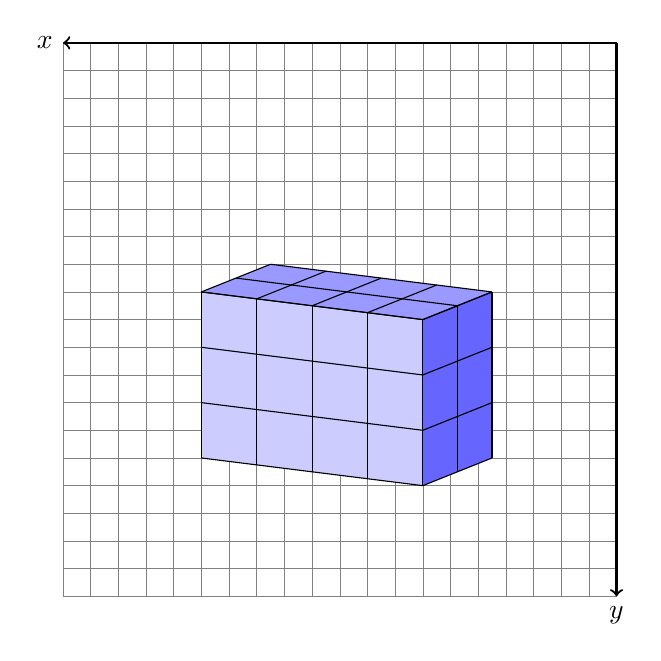
\begin{tikzpicture}
    \draw[help lines, step=1em] (0,0) grid (-20em, -20em);
    \draw[thick, ->] (0,0) -- (-20em, 0) node[left] {$x$};
    \draw[thick, ->] (0,0) -- (0, -20em) node[below] {$y$};
    
    \def\xsize{2};
    \def\ysize{3};
    \def\zsize{4};
  
    \begin{scope}[shift={(-15em, -15em)}, x={(2em,-0.25em)},y={(0em,2em)}, , z={(-1.25em,-0.5em)}]
      % Draw the front face
      \fill[blue!20] (0,0,0) -- (0,\ysize,0) -- (\zsize, \ysize,0) -- (\zsize,0,0) -- cycle;
      % Draw the top face
      \fill[blue!40] (0,\ysize,0) -- (0,\ysize,-\xsize) -- (\zsize, \ysize, -\xsize) -- (\zsize, \ysize,0) -- cycle;
      % Draw the right face
      \fill[blue!60] (\zsize,0,0) -- (\zsize,0,-\xsize) -- (\zsize, \ysize, -\xsize) -- (\zsize, \ysize,0) -- cycle;
  
      \foreach \x in {0,1, ..., \xsize}
      {
        \draw[black] (0, \ysize, -\x/\xsize * \xsize) -- (\zsize, \ysize, -\x/\xsize * \xsize);
        \draw[black] (\zsize,0,-\x/\xsize * \xsize) -- (\zsize, \ysize,-\x/\xsize * \xsize);
      }
  
      \foreach \y in {0, 1, ..., \ysize}
      {
        \draw[black] (0,\y/\ysize * \ysize,0) -- (\zsize,\y/\ysize * \ysize,0);
        \draw[black] (\zsize,\y/\ysize * \ysize,0) -- (\zsize,\y/\ysize * \ysize,-\xsize);
      }
  
      \foreach \z in {0, 1, ..., \zsize}
      {
        \draw[black] (\z/\zsize * \zsize,\ysize,0) -- (\z/\zsize * \zsize,\ysize,-\xsize);
        \draw[black] (\z/\zsize * \zsize,0,0) -- (\z/\zsize * \zsize,\ysize,0);
      }
    \end{scope}
  \end{tikzpicture}
  \caption{An example of MPI Cartesian topology Scheme of $24$ processors.}
  \label{FIG_MPI_TOPOLOGY_24_PROCS}
\end{figure}

\paragraph{Determine MPI datatypes for communication}
In order to do MPI communications, the source and the destination of every process are necessary, also the datatype.
When working with the meta-designed multidimensional matrix, we need to utilize the function \texttt{MPI\_Type\_Create\_subarray} to 
create essential halo datatypes.
\begin{algorithm}
  \begin{algorithmic}[1]
    \STATE \texttt{array\_size}, \texttt{array\_subsize}, \texttt{array\_starts=\{0\}} \hfill \#\texttt{std::array<Integer, NumD>}, the information of matrix.
    \FOR {i = 0 : NumD}
      \STATE Split tasks in dimension \texttt{i} by calling \texttt{decomposition}
      \STATE \texttt{array\_size = }local shape
      \STATE \texttt{array\_subsize = array\_size - 2}
    \ENDFOR
    \FOR {i=0 : NumD}
      \STATE \texttt{temp = array\_subsize[i]} \hfill \# Store the number temporally.
      \STATE \texttt{array\_subsize[i] = 1}
      \STATE \texttt{MPI\_Type\_Create\_subarray
      } and \texttt{MPI\_Type\_commit()} \hfill \# Create halo in dimension \texttt{i} and commit.
      \STATE Restore temporal array sub-size.
    \ENDFOR
  \end{algorithmic}
\end{algorithm}

\begin{figure}[htbp]
  \centering
  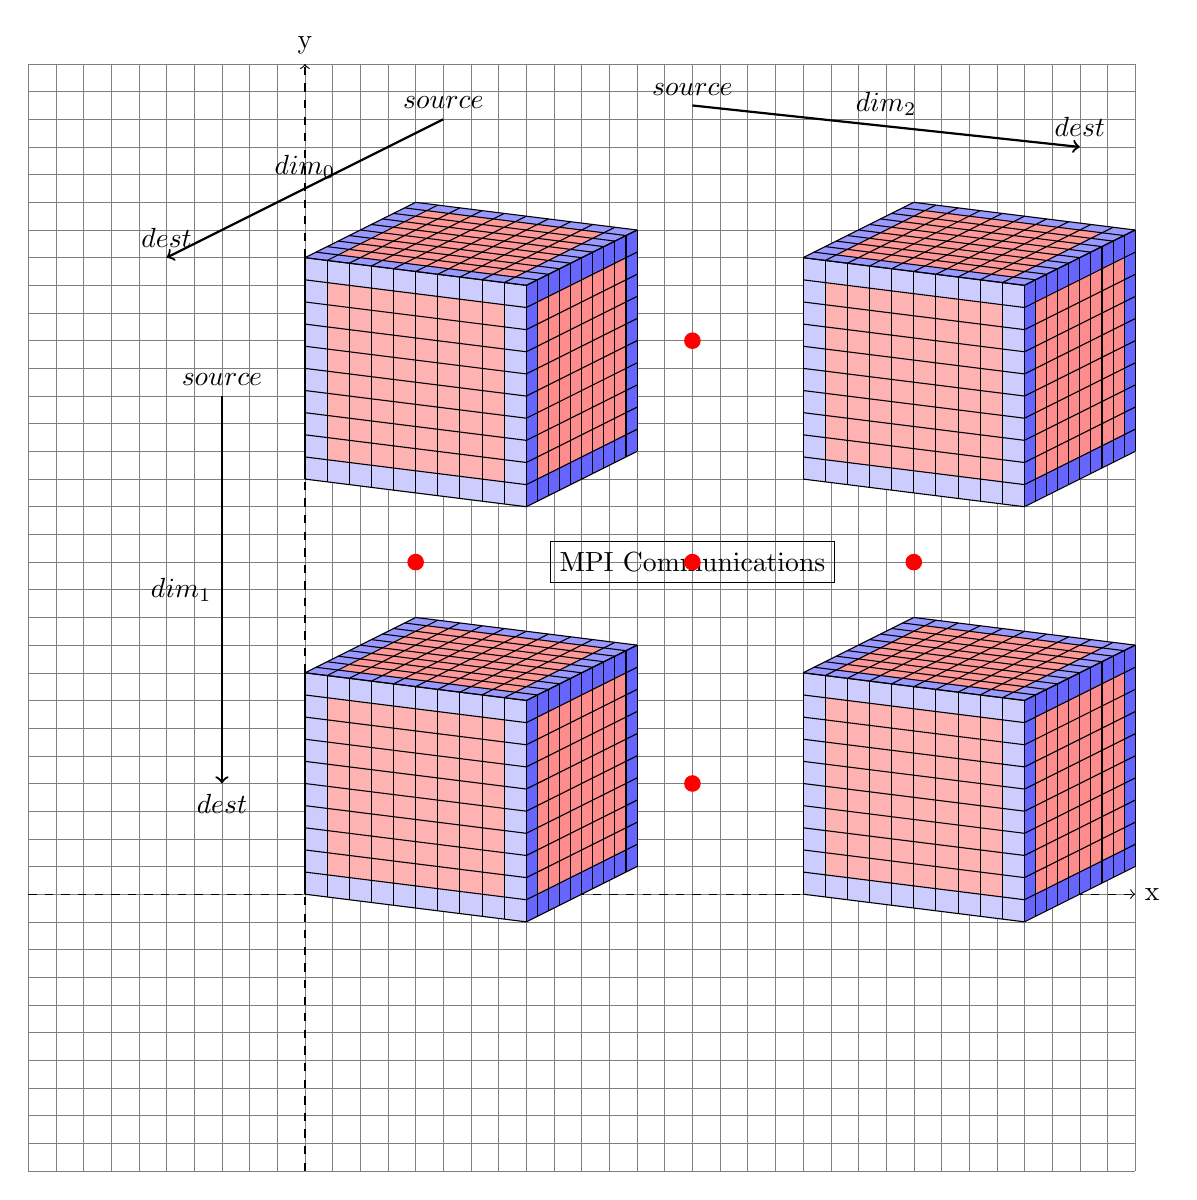
\begin{tikzpicture}
    % Draw a grid with steps of 1 cm
    \draw[help lines, step=1em] (-10em,-10em) grid (30em,30em);
  
    % Draw axes
    \draw[dashed,->] (-10em,0) -- (30em,0) node[right] {x};
    \draw[dashed,->] (0,-10em) -- (0,30em) node[above] {y};
  
    \draw[thick,->] (5em, 28em) -- (-5em, 23em) node[pos=0, above] {$source$} node[pos=0.5, above] {$dim_0$} node[pos=1, above] {$dest$};
    \draw[thick,->] (-3em, 18em) -- (-3em, 4em) node[pos=0, above] {$source$} node[pos=0.5, left] {$dim_1$} node[pos=1, below] {$dest$};
    \draw[thick,->] (14em, 28.5em) -- (28em, 27em) node[pos=0, above] {$source$} node[pos=0.5, above] {$dim_2$} node[pos=1, above] {$dest$};
  
      % Define a local macro to draw a cube at a given position
      \def\drawcube#1#2{
        \begin{scope}[shift={#1}, x={(0.8em,-0.1em)}, y={(0em,0.8em)}, z={(0.4em,0.20em)}]
          \def\size{#2}
          % Draw the front face
          \fill[blue!20] (0,0,0) -- (0,\size,0) -- (\size, \size,0) -- (\size,0,0) -- cycle;
          % Draw the top face
          \fill[blue!40] (0,\size,0) -- (0,\size,\size) -- (\size, \size, \size) -- (\size, \size,0) -- cycle;
          % Draw the right face
          \fill[blue!60] (\size,0,0) -- (\size,0,\size) -- (\size, \size, \size) -- (\size, \size,0) -- cycle;
  
          \fill[red!30] (1,1,0) -- (1,\size-1,0) -- (\size-1, \size-1,0) -- (\size-1,1,0) -- cycle;
          \fill[red!40] (1,\size,1) -- (1,\size,\size-1) -- (\size-1, \size, \size-1) -- (\size-1, \size,1) -- cycle;
          \fill[red!45] (\size,1,1) -- (\size,1,\size-1) -- (\size, \size-1, \size-1) -- (\size, \size-1,1) -- cycle;
  
          % Draw the grid
          \foreach \x in {0,1,...,\size} {
            \draw[black] (\x,0,0) -- (\x,\size,0);
            \draw[black] (0,\x,0) -- (\size,\x,0);

            \draw[black] (\size,\x,0) -- (\size,\x,\size);
            \draw[black] (\size,0,\x) -- (\size, \size,\x);

            \draw[black] (\x,\size,0) -- (\x,\size,\size);
            \draw[black] (0,\size,\x) -- (\size, \size,\x);
          }
        \end{scope}
      }
  
      % Draw the first cube at (0,0) with size 8
      \drawcube{(0em, 0em)}{10}
      \drawcube{(18em, 0em)}{10}
      \drawcube{(0em, 15em)}{10}
      \drawcube{(18em, 15em)}{10}
        
      \node[draw, minimum width = 3em, minimum height = 1.5em, align=center] at (14em,12em) {MPI Communications};
    
      \fill[red] (14em,12em) circle (3pt);
      \fill[red] (14em,4em) circle (3pt);
      \fill[red] (14em,20em) circle (3pt);

      \fill[red] (4em,12em) circle (3pt);
      \fill[red] (22em,12em) circle (3pt);
    \end{tikzpicture}  
  \caption{A 3D MPI Communication Scheme of $8$ processors between $3$ dimension matrices.}
  \label{FIG_MPI_3D_Example_SCHEME}
\end{figure}


\subsection{Template Distributed Multi-dimension Matrix Design}
\subsubsection{Detail Object Design}
Adhering to the STL safety routines, I chose to create detail template class object, hidden from users,
named \texttt{\_\_array\_Cart<class \_\_T, \_\_size\_type \_\_NumD>}.
Here, the \texttt{\_\_T} represents the value type, \texttt{\_\_size\_type} specifies the type of number of dimensions.
Since it is internal and not exposed from users, I decided to directly use other detail objects as member variables rather than 
smart pointers.
In this context, Cartesian matrix has public member variables \texttt{\_\_array} and \texttt{topology::Cartesian},
and provides memory operations. 
But the copy, move constructors and assignment operators are removed.
This approach enhances both performance both performance and simplicity by avoiding unnecessary abstractions in the internal design 
while maintain a robust memory management.

\paragraph{Distributed operator <<}
The STL os stream operator \texttt{<<} prints the matrices of all processes in sequence which build on multidimensional matrix's. 
Thus the Unix standard \texttt{fflush} function is utilized for flushing the cache in terminal, to ensure the stdout is print immediately.

\subsubsection{User Interface Design}
The \texttt{array\_Cart<class T, size\_type NumD>} is an object exposed to users, whereas only provides limited access to member variables by smart pointer.
As the size of matrices stored, it becomes clear that memory management is critically important. 
Secondly, especially in MPI distributed matrices, exposing direct memory access by set it to public member is dangerous. 
With the profits mentioned in Section \ref{SEC:RAII}, using unique pointer brings more benefits in this scenario, 
\begin{enumerate}
  \item MPI program memory management has higher complexity level. 
  Adhering RAII routines, the resources are bind with object, including MPI objects, and will be deleted as the object destructed. 
  \item Simplifying Concurrency Control. Synchronization between processes is a critical issue. 
  By using the RAII, user could unsure the resources are locked or released automatically, preventing the risk of deadlocks and resource contention.
\end{enumerate}



\subsection{Template Function Gather of Cartesian Distributed Multi-dimension Matrix}
% \subsubsection{Pure Message Passing Parallel}
% \subsubsection{Hybrid Parallel}

\subsection{Physics Informed Neural Networks}
\subsubsection{CUDA parallel}
\subsubsection{Hybrid Parallel}
\section{Experiments}
\subsection{Experimental Setup}


I verify the proposed PINN methods on generated dataset, and FDTD methods with hybrid and pure MPI strategies
on the server with two Intel (R) Xeon (R) Platinum 9242 CPU nodes (96 cores per node) and $4$ NUMA nodes per node.
While the dataset is using \texttt{std::m19937} STL random device with given seed $42$ \cite{STL:RANDOM_SEED}.
The PINN models I mentioned are trained using train-from-scratch strategy, and maximin number of training times is $1'000'000$ epochs.
In the setting of learning rate and optimizer, I chose to use Adam with constant learning speed $10^{-3}$.
The details of PDEs are determined in previous section \ref{SEC:Specific_Form}.  

\paragraph{Compiling}
Compiling the program is also a critical important processes.
I chose to use the macros for defining the scale of problems in advance, this is because the compiler will 
have more aggressive optimizations if it knows more predefined parameters.

\paragraph{Running}
For finely manipulate the resource allocation on cluster, following command line \ref{LST:mpirun} is used for this 
the script arguments \texttt{rsc} stands for the resource type such as \texttt{numa}, \texttt{node} and \texttt{socket},
\texttt{--report-bindings} is a error message, for showing the details of threads and CPUs tasks allocated on cluster.
\begin{lstlisting}[
  style=customCpp,
  caption={main command line for launching program on cluster},
  label={LST:mpirun}]
    mpirun --map-by ppr:$ppr:$rsc:pe=$threads --report-bindings <executable> <arguments>
\end{lstlisting}
and \texttt{threads} means the number of threads per resource. The \texttt{ppr} is the number of CPU tasks per resource.
The last \texttt{<argument>} is command line arguments for the program, which is designed by programmer. 
In this case, I designed three type of arguments
\begin{enumerate}
  \item \texttt{-S, -s} Strategy, for specifying the pure mpi, hybrid 0 or 1 strategy.
  \item \texttt{-F, -f} file name, if this argument is defiend, the results will be stored in the file.
  \item \texttt{-H, -h} Helper message, the usage information.
  \item \texttt{-V, -v} Showing the version of program.
\end{enumerate}



\subsubsection{Computational Topology}
The computational topology is critically important when we are programming parallel PDEs solver softwares.
Put the strongly speed-dependent data into the slow memory could make entire program slower.

\paragraph{Cluster}
The cluster we are using for this project is \texttt{Callan} \cite{Callan_TCD} which has 
$2$ CPUs per compute node, and each CPU has $32$ cores with single thread. 
The Non-Uniform Memory Access (NUMA) nodes are layout as following 
\begin{figure}[htbp]
  \centering
  \begin{tikzpicture}[scale=0.8, transform shape]
    \node[anchor=south west,inner sep=0] (image) at (0,0) {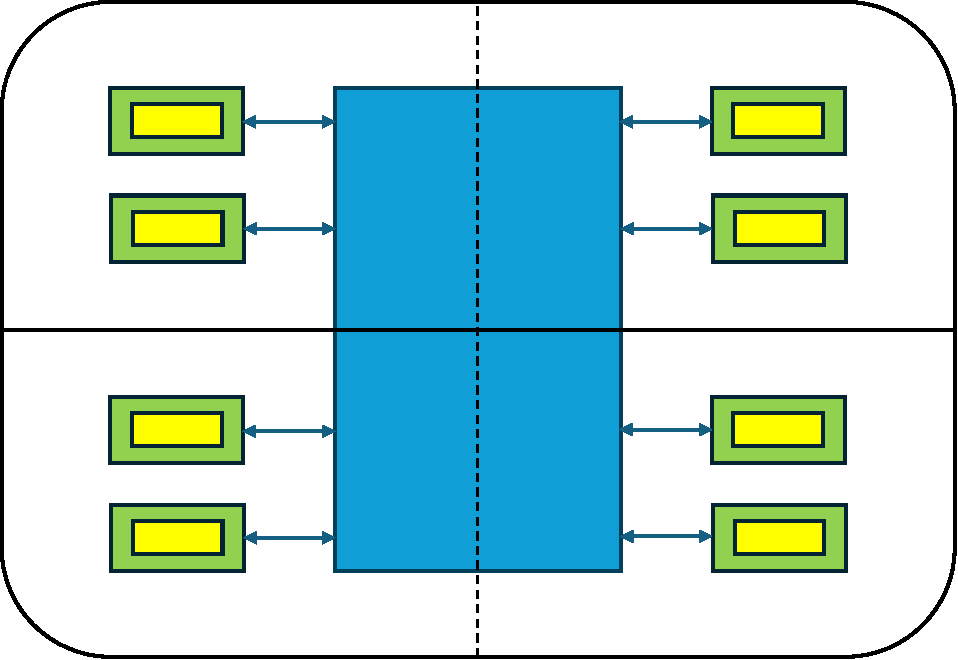
\includegraphics[width=0.5\textwidth]{figure/FIG_Topology_9242.pdf}};
    % \node[anchor=south west,inner sep=0] (image) at (0,0) {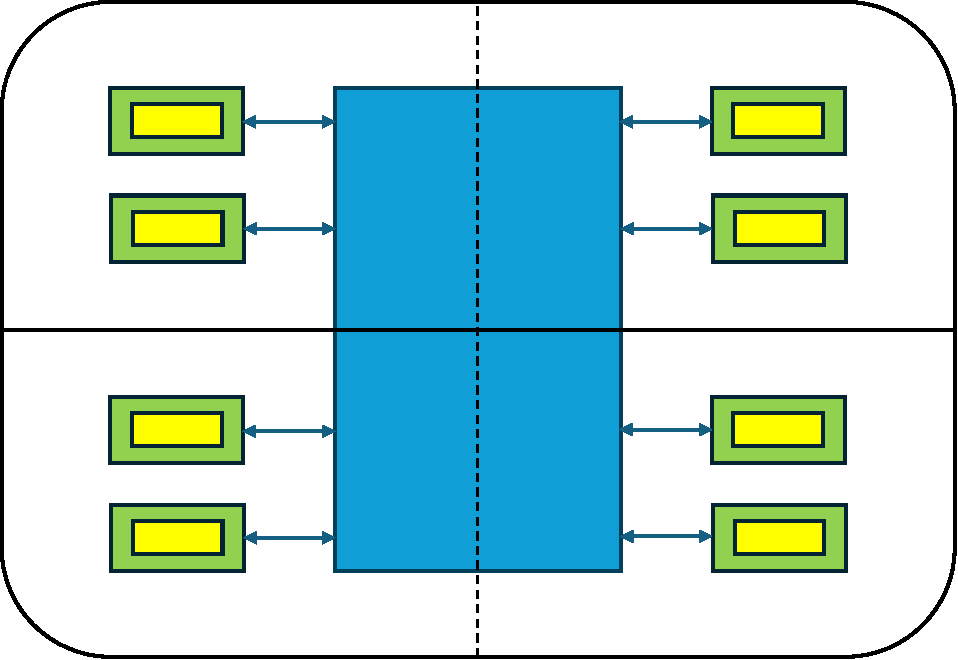
\includegraphics[width=0.58\textwidth]{figure/FIG_Topology_9242.pdf}};     /// overleaf
    \begin{scope}[x={(image.south east)},y={(image.north west)}]
        % \draw[help lines, step=1em] (-1em,-1em) grid (30em,20em);    
        % % Draw axes
        % \draw[dashed,->] (-1em,0) -- (30em,0) node[right] {x};
        % \draw[dashed,->] (0,-1em) -- (0,20em) node[above] {y};

      \node at (12em,18em) {$2$ $Scokets$};

      \node at (4.5em,1em) {$DDR4$};
      \node at (19.5em,1em) {$DDR4$};

      \node at (4.5em, 15em) {$DDR4$};
      \node at (19.5em,15em) {$DDR4$};

      \node at (12em,13em) {Hyper-threads};
      \node at (12em,5.5em) {Hyper-threads};

      \node at (12em,11em) {$48$ $CPUS$};
      \node at (12em,3.5em) {$48$ $CPUS$};
    \end{scope}
  \end{tikzpicture}
  \caption{NUMA topology of single node on Cluster}
  \label{FIG_Topology_Callan}
\end{figure}
Accessing the other NUMA node's memory reduces the bandwidth and also the latency,
though the bandwidth is commonly high enough, the latency can increase by 
$~30\%$ to $~400\%$ \cite{NUMA_Latency_TCD}. 
This latency becomes dangerous when writing shared memory parallel programs.


\subsection{Comparison on single node}
On single node, the CPUs are connected by high-bandwidth, low-latency internal bus which is faster than connection between nodes.
However, for the $4$ total NUMA nodes per compute node, memory accessing between them has higher latency than cache.
Thus, the first tests set were run on the platform with single node, to evaluate the parallelistic performance of heat equation on 2 and 3 dimension spaces with 
3 strategies.


\subsubsection{Strong Scaling}
Figure \ref{FIG:Benchmark:PURE_MPI} visualizes the comparison of my proposed parallelistic program using pure MPI on two dimension space heat euqation with 
the number of CPUs and various problem scales.
Overall, the more CPUs brings more performance among all scales from $512^2$ to the $32'768^2$ but can not break the speedup limits.
Compared with large scale bigger than $4096^2$, the light problems has less speedup as the number of CPUs increases.
By seeing the trend of speedup ratios drop as the CPU gets more, 
the trend can be readily discovered which is the as the scale of problems gets larger, the latter it will have performance-dropping.
Once the problem size is large enough, ($4096^2$ and larger), the solvers can get the more benefits from more CPUs.

\begin{figure}[htbp]
  \centering
  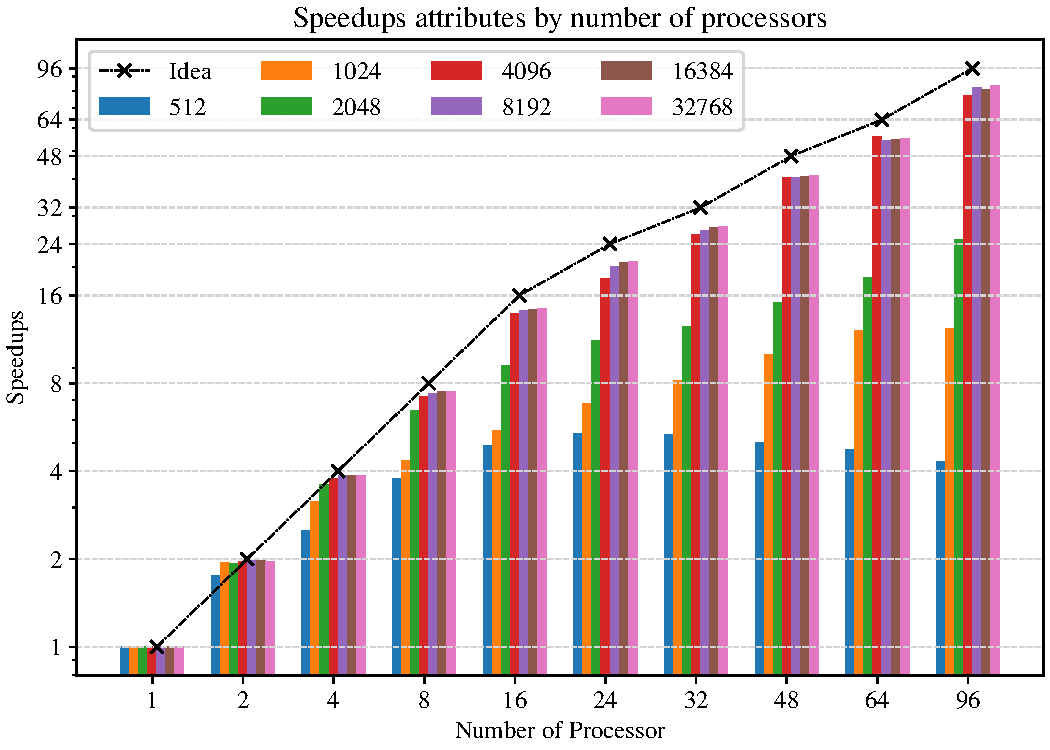
\includegraphics[width=0.6\textwidth]{figure/FIG_Benchmark_pure_mpi.pdf}
  \caption{
    Comparison of speedup ratios of strong scaling tests of pure MPI parallelized program. 
    The investigated problem scales are the power of $2$, exponents ranging from $9$ to $15$.
    The number of CPUs are also set as power of $2$, with additional numbers $24$, $48$ and $96$ matched the topologies of CPU.
  }
  \label{FIG:Benchmark:PURE_MPI}
\end{figure}

On the other hand, I also include some unconventionaly number of CPUs in scaling tests such as $24$, $48$ and $96$ for comparison. and 
the results are also shown in the figure \ref{FIG:Benchmark:PURE_MPI}.
From this figure, it is hard to tell the difference of these where it ought to indicate some information about its NUMA structure.
This is because the MPI communication does not strongly effected by memory structure, while the hybrid does.
Figure \ref{FIG:Benchmark:Hybrid} shows the difference, the hybrid strategy brings lower performance with small scale across all CPUs and 
approximately identical in the large scale cases.
The most visible change in figure \ref{FIG:Benchmark:Hybrid_0} is that the speedup ratio of problem with scale $4096^2$ 
exceded the limits on $4$, $8$ and $16$ CPUs which is $1$, $2$, $4$ threads of each MPI process.
We can also see that when the number of threads is $8$ and $4$ MPI processes, the performances on large scale is better than pure MPI parallelism.

\begin{figure}[htbp]
  \centering
  \subfigure[No overlapping comm./comp.]
  {
    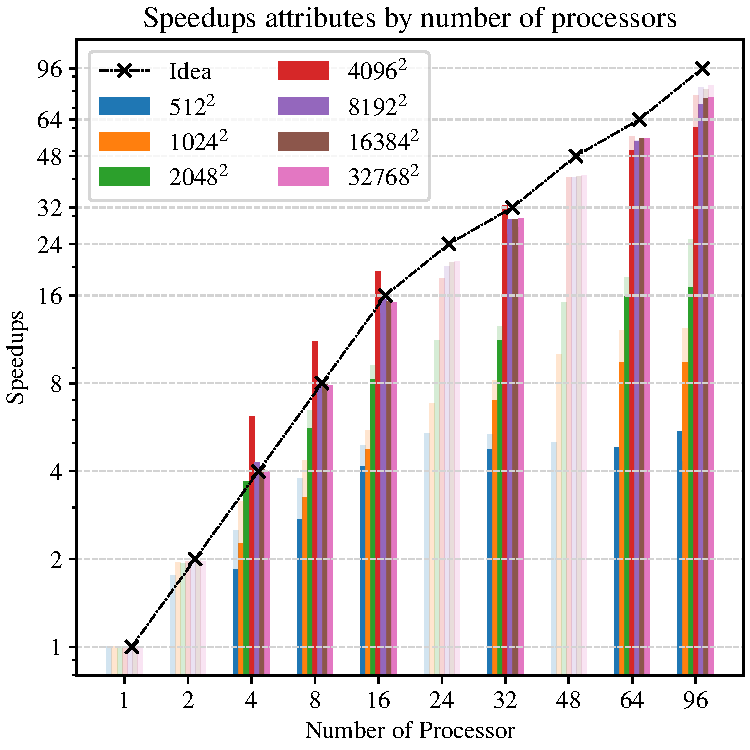
\includegraphics[width=0.47\textwidth]{figure/FIG_Benchmark_hybrid_0.pdf}
    \label{FIG:Benchmark:Hybrid_0}
  }
  \hfill
  \subfigure[With overlapping comm./comp.]
  {
    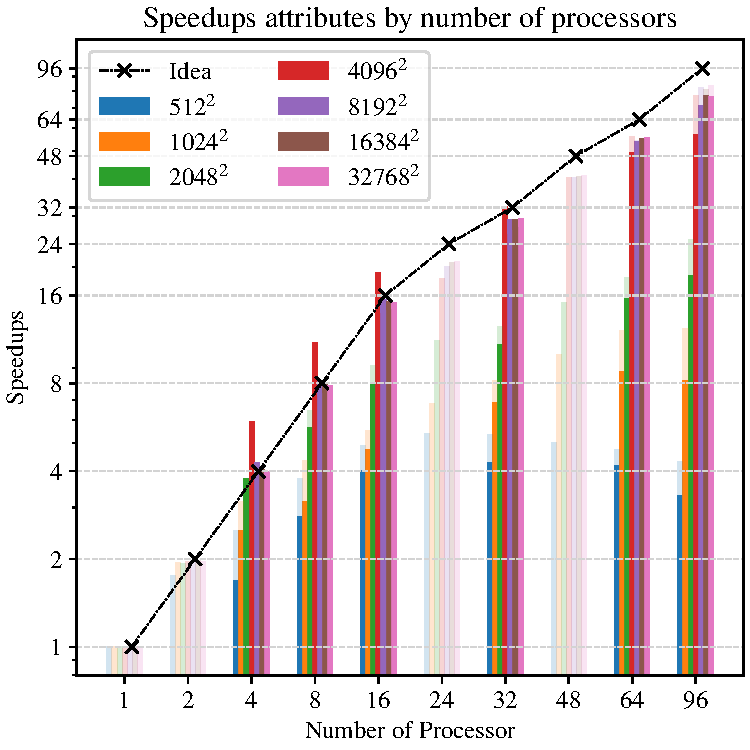
\includegraphics[width=0.47\textwidth]{figure/FIG_Benchmark_hybrid_1.pdf}
    \label{FIG:Benchmark:Hybrid_1}
  }
  \caption{
    Comparison of speedup ratios of strong scaling tests of mater-only parallelized program with overlapping and no overlapping of computation and communication.  
    The vague background is the results of pure MPI parallelization from figure \ref{FIG:Benchmark:PURE_MPI} and problems sclaes are identical as well.
    The number of threads are set to $1$, $2$, $4$, $8$, $16$, and $24$, 
    tasks per CPU are $1$, $2$ and $4$.
  }
  \label{FIG:Benchmark:Hybrid}
\end{figure}

For the other funneled hybrid parallelization, the figure 
            \ref{FIG:Benchmark:Hybrid_1} 
in the appendix shows the details of results,
this strategy has nearly idential performance of master only with no overlapping on large problem scales.
However, the behaviour of it on small scales has a different pattern.
This indicates that the overlappings of computation and communication are not as good as previous one, which means the overload management is not 
well on these tests.


\paragraph{Superliner Speedup}
Conventionally, the actuall speedup won't excedes the theoratical predictions of Amdalh's law.
However, the scaling of two hybrid programs did exceded the limits but exclusively on the problem scale $4096^2$ and $1$ to $8$ threads of each $4$ MPI processes.
Considering the details of the CPU used for these tests, 
\begin{itemize}
  \item It has $4$ NUMA node per CPU and once of which has $12$ CPUs with $2$ threads.
  \item It has \texttt{32KB} L1 data and L1 instruction cache, \texttt{1024KB} L2 cache and \texttt{36608KB} L3 cache.
\end{itemize}
The data type for this solver is \texttt{Double} which takes $8$ bytes, and $4096^2$ \texttt{Double} numbers takes 128 \texttt{MB} to store.
In the case of $4$ MPI processes, each process own a quater of number which uses 32 \texttt{MB} for handling sub-problems.
On the other hand, the L3 cache is 36608 \texttt{KB} = 35.75 \texttt{MB} which is just bigger than the sub-problem scale 32 \texttt{MB}.
When the problem size gets larger, such as $8096^2$ which takes 128 \texttt{MB} to store the sub-problem. 
In such case, the L3 case is no longer able to hold it, thus part of the numbers will be stored in the DDR4 memories which is lower bandwidth and higher latency than cache.
Moreover, due to the CPU enables hyper-threading, a NUMA node actually holds $12$ CPUs, which makes the 
superlinear speedup disappear when the threads is 16 and 24.

% \begin{figure}[htbp]
%   \centering
%   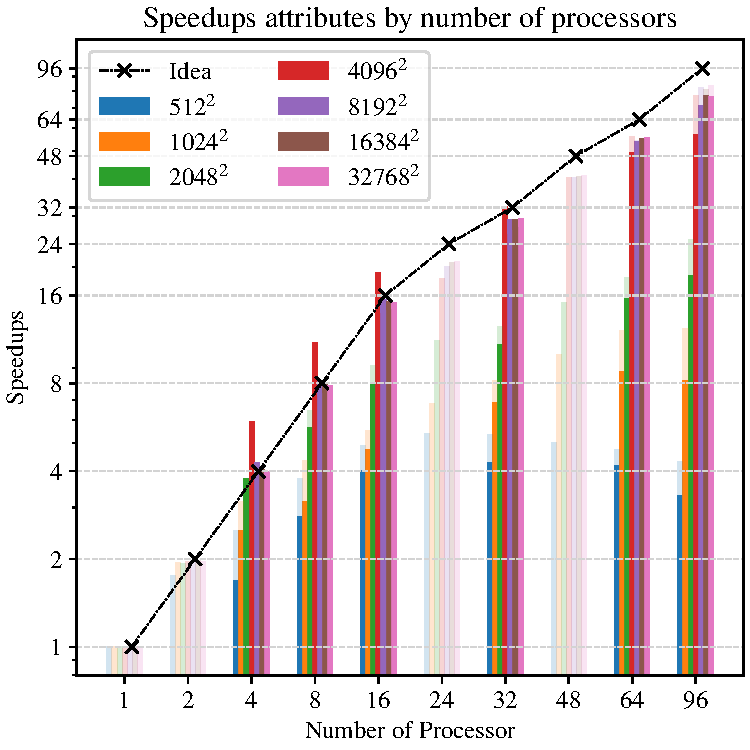
\includegraphics[width=0.7\textwidth]{figure/FIG_Benchmark_hybrid_1.pdf}
%   \caption{<caption>}
%   \label{FIG:Benchmark:Hybrid_1}
% \end{figure}

% \begin{figure}[htbp]
%   \centering
%   \subfigure[Grid sizes: 150*45*40/25*33*40.]{
%       \includegraphics[width=0.45\textwidth]{weak.png}
%       \label{fig:weak_scaling_1}    
%   }
%   \hfill
%   \subfigure[Grid sizes: 300*90*80/50*65*80]{
%       \includegraphics[width=0.48\textwidth]{weak_scaling_2_efficiency_comparison.png}    
%       \label{fig:weak_scaling_2}
%   }
%   \caption{
%       Weak scaling tests of Cartesian / Cylinder equation with same problem scale on $1$, $2^2$, $3^3$, $4^3$ processors.
%   }
%   \label{fig:weak_scaling}    
% \end{figure}

\subsubsection{Weak Scaling}\label{SSS:Weak_Scaling:SingleNode}

Table \ref{TAB:Benchmark:Weak_PURE_MPI} lists the weak scaling comparison of three different parallel strategies.
Overall, both three strategies have good weak scaling results across all problem sizes.
For example, according to the Gaustafsson's Law \ref{THEO:GaustafssonLaw}, the program using
overlapped strategy has sequential fraction 
$$f_s = \frac{49.989 - 64}{1-63} \approx 0.222$$
on the problem scale $4096^2$ with 64 CPUs
and $f_s \approx 0.147$ with 16 CPUs.
For the small size problems, like $512^2$, the pure MPI has significantly higher weak scaling efficiency comparing to the other two,
more specifically about $7.8\%$, $7.5\%$ higher in 64, 16 CPUs, and $22.5\%$ higher in 4 CPUs.
However, as the scale gets larger, this advantages gradually disappear and even worse than other two.
Especially when $4096^2$ on 16 and 64 cores, the forward leap of hybrid versions gets larger, about $34.4\%$ and $28.1\%$ higher than 
pure MPI respectively.

On the other hand, the superlinear speedup appears for the problem size with $512^2$ and $1024^2$ on 4 CPUs.
This is because the sub-problem for each CPUs only take 512 \texttt{KB} and 1024 \texttt{KB} to store, 
which is the L2 cache size of the Xeon Platinum 9242.
Thus the four processes could take the performance advantages of L2 cache individual for each CPU.
Once the problem size gets larger, such as $2048^2$, part of the problem will be allocated on L2 cache and other parts on L3 cache.
These memory allocations requires extra synchronization between cache accessing, which drop the performance down.
However, as the size gets to $4096^2$, the sub-problem will be fully make use of L3 cache, which require less synchronization of cache, 
the weak scaling goes up but we can not see the superlinear speedup again.

\begin{table}
  \caption{Weak Scaling on Single Node of 2D Heat Equation}
  \label{TAB:Benchmark:Weak_PURE_MPI}
  \begin{minipage}{\columnwidth}
    \begin{center}
      \footnotesize % overleaf
      \begin{tabular}{>{\bfseries}p{3cm} p{1.5cm} p{1.5cm} p{1.5cm} p{1.5cm} p{1cm}}
        \toprule
        \multirow{2}{*}{Strategy}     & \multirow{2}{*}{\bfseries Size} & \multicolumn{3}{c}{\bfseries  Number of CPUs}   & \multirow{2}{*}{\bfseries $f_p(\%)$}  \\
                                      &                                  & \bfseries 4   & \bfseries 16   & \bfseries 64  &                                       \\
        \midrule
        Pure MPI      & \multirow{3}{*}{$512^2$}      & 4.006  & 12.497  & 47.849                                         & 75.1 \\
        No Overlap    &                               & 2.876  & 11.206  & 42.754                                         & 67.0 \\
        With Overlap  &                               & 3.173  & 10.818  & 42.282                                         & 66.2 \\
        \midrule
        Pure MPI      & \multirow{3}{*}{$1024^2$}     & 3.838  & 9.304   & 33.707                                         & 53.2  \\
        No Overlap    &                               & 3.947  & 12.995  & 33.447                                         & 54.1 \\
        With Overlap  &                               & 4.024  & 12.932  & 33.361                                         &  54.0 \\
        \midrule
        Pure MPI      & \multirow{3}{*}{$2048^2$}     & 2.376  & 8.245   & 31.203                                         &  49.0\\
        No Overlap    &                               & 3.874  & 8.972   & 31.510                                         &  49.8 \\
        With Overlap  &                               & 3.740  & 8.989   & 31.430                                         &  49.7 \\
        \midrule
        Pure MPI      & \multirow{3}{*}{$4096^2$}     & 3.543  & 8.245   & 31.203                                         &  77.5\\
        No Overlap    &                               & 3.953  & 13.799  & 49.515                                         &  78.0\\
        With Overlap  &                               & 3.948  & 13.800  & 49.989                                         &  78.7 \\
        \bottomrule
      \end{tabular}
    \end{center}
    % \bigskip
    % \footnotesize\emph{Source:} This is source 
  \end{minipage}
\end{table}

Moreover, since Gaustafsson' theorem \ref{THEO:GaustafssonLaw} gives us a linear module for valuating the parallel problem.
Thus I chose to use the linear model from equation \ref{EQ:GaustafssonLaw} as a linear polymonimal fitting.
Considering the original point has to be on the line, which stantds for $f_s + f_p = 1$, 
I manually create an extended version of speedups by concatenate a inverse negative one to ensure their 
means are $0$ which makes the fitting line across the $(0,0)$. 
Eventually, the results of $f_p$ are shown in the table \ref{TAB:Benchmark:Weak_PURE_MPI} as well.
These fitting lines also indicate that the hybrid parallelized versions has more parallel fraction than pure MPI when the scale of problem gets larger than $512$,
which means that hybrid strategies reduced the cost of synchronization and brought higher efficiency.



\subsection{Comparison on multi-node}
Running programs on multi-node also utilized the command line \ref{LST:mpirun} to specify the resource allocation on cluster.
In this setup, I ran the tests on $4$ nodes with total $16$ NUMA nodes or $384$ CPUs, all other settings are maintained from the single-node tests.
\subsubsection{Strong Scaling}
Figure \ref{FIG:Benchmark:PURE_MPI_Multi_Node} demonstrates speedup ratio of all candidates for test and their relationships with the number of CPUs.
In the big picture, it is easy to determine that the small scale problems (smaller than $4096^2$) had pool speedup performances on these settings.
Especially for the $512^2$, $1024^2$ and $2048^2$, parallelization even brought worse performance in the end, which is 
strongly different from the big scales.
In the large scale problems, the most large two maintained good strong scaling performances at the end, but 
the pure MPI failed on launching the program when using $384$ processes.
Moeover, the problem with $4096^2$ numbers show superlinear speedup on $4$, $8$ and $16$ processes which 
is similar to single-node hybrid tests.
However, unlike gaining benefits from shared memory operations on single NUMA node, 
these superlinear speedup came from the node structure.
Where the pure MPI processes were allocated on four different CPU, which has individual CPU clock cycle.
Thus, the processes can behave like operating on shraed memory model.
\begin{figure}[htbp]
  \centering
  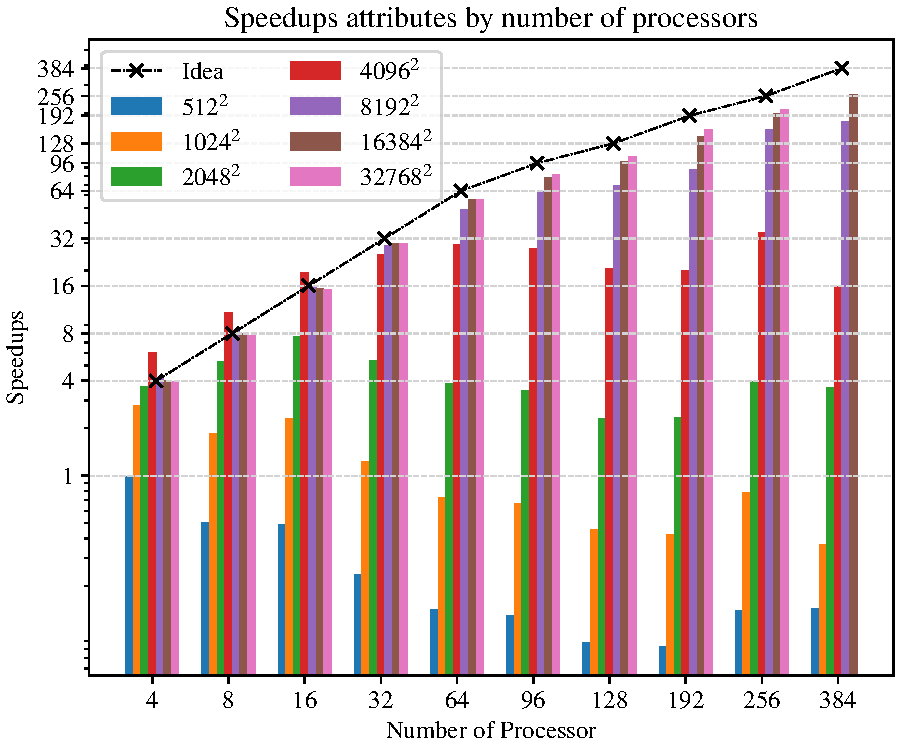
\includegraphics[width=0.55\textwidth]{figure/FIG_Benchmark_pure_mpi_multi_nodes.pdf}
  \caption{
    Comparison of speedup ratios of strong scaling tests of pure MPI parallelized program. 
    The investigated problem scales are the power of $2$, exponents ranging from $9$ to $15$.
    The number of CPUs are also set as power of $2$, with additional numbers $96$, $192$ and $384$ matched the topologies of CPU.
  }
  \label{FIG:Benchmark:PURE_MPI_Multi_Node}
\end{figure}
In addition, the patterns of the strong scaling are different from the Amdalh'S law \ref{THEO:Amdalh's law} demonstrates.
Which has may visible exceptional performance decreases, due to the topologies of CPUs, especially when using 
$32$, $48$ and $96$ CPUs per node.

On the other hand, 
based on comparison of the strong scaling speedup ratios and the amount of resources,
two hybrid versions performed better than pure MPI parallel and the 
results are shown in the figure \ref{FIG:Benchmark:Hybrid_Multi_Node}.
From the figure \ref{FIG:Benchmark:Hybrid_0_Multi_Node} and \ref{FIG:Benchmark:Hybrid_1_Multi_Node},
we could see that the superlinear speedup appears on the scale $4096^2$ and $8019^2$ which are effected by 
the previously mentioned two reasons, the high performance local NUMA node shared memory and individual CPU clock cycle.
More specifically, $8092^2$ \texttt{Double} numbers takes $512$ \texttt{MB} to store, $128$ \texttt{MB} on each node and $32$ \texttt{MB} per NUMA node,
which just fits the L3 cache size.

\begin{figure}[htbp]
  \centering
  \subfigure[No overlapping comm./comp.]
  {
    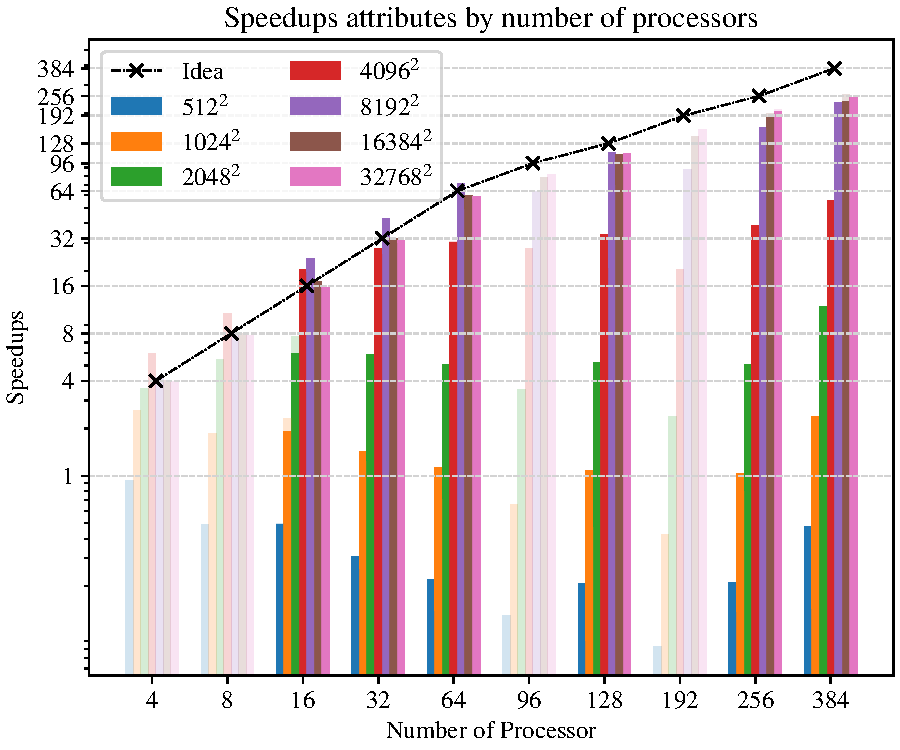
\includegraphics[width=0.47\textwidth]{figure/FIG_Benchmark_hybrid_0_multi_nodes.pdf}
    \label{FIG:Benchmark:Hybrid_0_Multi_Node}
  }
  \hfill
  \subfigure[With overlapping comm./comp.]
  {
    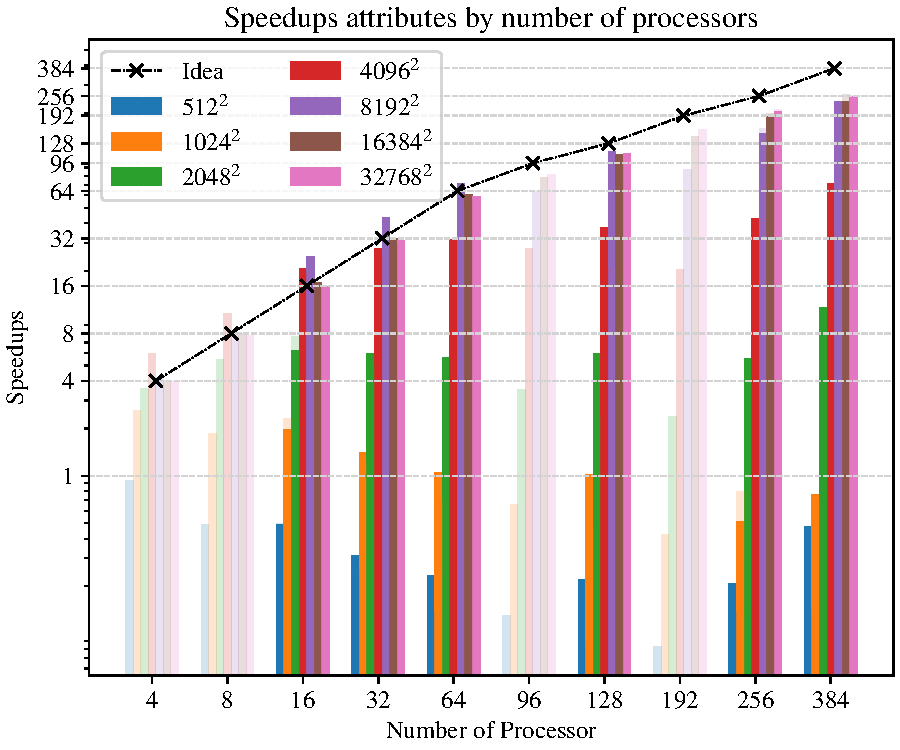
\includegraphics[width=0.47\textwidth]{figure/FIG_Benchmark_hybrid_1_multi_nodes.pdf}
    \label{FIG:Benchmark:Hybrid_1_Multi_Node}
  }
  \caption{
    Comparison of speedup ratios of strong scaling tests on $4$ nodes of 
    mater-only parallelized program with overlapping and no overlapping of computation and communication.  
    The vague background is the results of pure MPI parallelization from figure 
    \ref{FIG:Benchmark:PURE_MPI_Multi_Node} and problems sclaes are identical as well.
    The number of threads are set to $1$, $2$, $4$, $8$, $16$, and $24$, 
    tasks per CPU are $1$, $2$ and $4$.
  }
  \label{FIG:Benchmark:Hybrid_Multi_Node}
\end{figure}

As the amount of resources increase, the speedups are not increase as expected for all three parallel models.
However, hybrid parallel models were successfully launched on the $384$ CPUs, 
and also brought more performance for all tested number of CPUs.
These shows that the advantages of combination of shared memory programming and message-passing programming.

\subsubsection{Weak Scaling}

% PURE
% 512 48.185757348293464 [  3.29985789  10.37890476  25.99976339 124.37502699]
% 1024 49.30470677010394 [ 3.84763481 13.03676319 30.14287326]
% 2048 50.62289960989542 [ 3.7870875   9.17180313 32.01277006]
% 4096 80.22207174643209 [ 3.88441248 13.85932765 51.04086597]

% Hybrid 0
% 512 49.318336840965884 [  8.09445064  25.93147463 127.648308  ]
% 1024 69.80932598630608 [13.70192876 44.04014219]
% 2048 55.675781151306126 [13.93648546 34.36848416]
% 4096 83.806215053791 [15.31462331 53.15704013]

% Hybrid 1
% 512 45.51606462315708 [  8.38595555  27.12574758 116.95116903]
% 1024 69.93179786064245 [13.83401    44.09042189]
% 2048 55.86720303491557 [14.27434744 34.41421545]
% 4096 84.15726269711293 [15.29389611 53.40098918]
Table \ref{TAB:Benchmark:Weak_PURE_MPI_Multi_Node} lists the weak scaling comparison results of multi-node tests.
Overall, the hybrid models have better scaling speedup ratios than pure MPI model on the size larger than $512^2$.
Although the speedups of pure MPI model are better than hybrid models on $16$ CPUs with $2048^2$ problem size,
the hybrid model with no comm./comp. overlapping still have better performance when testing is running on $64$ and $256$ CPUs.
Controversially, the hybrid with no overlapping has better results comparing to the one with overlapping,
and we have opposite results when the scale gets larger.

On the other hand, similar to previous section \ref{SSS:Weak_Scaling:SingleNode}, the fraction of parallelizable is approximated by linder regression 
based on the model proposed in theorem \ref{THEO:GaustafssonLaw}.
As the table \ref{TAB:Benchmark:Weak_PURE_MPI_Multi_Node} lists results, the fraction of parallelizable increases as the size gets larger.
Moreover, the overlapping has the most large fraction then the model with no overlapping, and both of then are significantly larger than pure MPI model.

\begin{table}[htbp]
  \caption{Weak Scaling on Multi-node of 2D Heat Equation}
  \label{TAB:Benchmark:Weak_PURE_MPI_Multi_Node}
  \begin{minipage}{\columnwidth}
    \begin{center}
      \footnotesize % overleaf
      \begin{tabular}{>{\bfseries}p{3cm} p{1.5cm} p{1.5cm} p{1.5cm} p{1.5cm} p{1.5cm} p{1cm}}
        \toprule
        \multirow{2}{*}{Strategy}     & \multirow{2}{*}{\bfseries Size} & \multicolumn{4}{c}{\bfseries  Number of CPUs}   & \multirow{2}{*}{\bfseries $f_p(\%)$}  \\
                                      &                                 & \bfseries 4   & \bfseries 16   & \bfseries 64  & \bfseries 256  &                        \\
        \midrule
        Pure MPI      & \multirow{3}{*}{$512^2$}      & 3.300  & 10.379  & 26.000   & 124.375                                    & 48.2 \\
        No Overlap    &                               &   -    &  8.094  & 25.931   & 127.648                                    & 49.3 \\
        With Overlap  &                               &   -    &  8.386  & 27.126   & 116.951                                    & 45.5 \\
        \midrule
        Pure MPI      & \multirow{3}{*}{$1024^2$}     & 3.848  & 13.037  & 30.143   &   -                                        & 49.3 \\
        No Overlap    &                               &   -    & 13.702  & 44.040   &   -                                        & 69.8 \\
        With Overlap  &                               &   -    & 13.834  & 44.090   &   -                                        & 69.9 \\
        \midrule
        Pure MPI      & \multirow{3}{*}{$2048^2$}     & 3.787  & 9.172   & 32.013   &   -                                        & 50.6 \\
        No Overlap    &                               &   -    & 13.936  & 34.368   &   -                                        & 55.7 \\
        With Overlap  &                               &   -    & 14.274  & 34.414   &   -                                        & 55.9 \\
        \midrule
        Pure MPI      & \multirow{3}{*}{$4096^2$}     & 3.884  & 13.859  & 51.041   &   -                                        & 80.2 \\
        No Overlap    &                               &   -    & 15.315  & 53.157   &   -                                        & 83.8 \\
        With Overlap  &                               &   -    & 15.294  & 53.401   &   -                                        & 84.2 \\
        \bottomrule
      \end{tabular}
    \end{center}
    % \bigskip
    % \footnotesize\emph{Source:} This is source 
  \end{minipage}
\end{table}

There are some important performance leap forward 
due to the memory structure mentioned in previous section \ref{SSS:Weak_Scaling:SingleNode}, the L3 cache for single NUMA node 
just fits the problem with $2048^2$ \texttt{Double} numbers.
\begin{itemize}
  \item The first one is the number of CPUs increases from $16$ to $64$, in the case of the problem size is $1024^2$ running on hybrid models, 
  the problem scale of each NUMA node increases from $1024^2$ to $2048^2$ which makes the program requires less cache synchronization 
  and brings about $52.6\%$ more scaling speedup performance.
  \item The second is the size of problems increas from $1024^2$ to $2048^2$ when the number of CPUs is $16$.
  With such doubled size, the program can make more use of L3 cache on single NUMA node and brings about speedup $46.6\%$ improvements. 
\end{itemize}
Both of the improvements are about $50\%$, these results indicates that the hybrid strategies I was implementing are effective, 
also, the overlapping of computation and communication promoted the 
speedup further.

\subsection{Comparison on Dimension}
\subsubsection{Strong Scaling}
The figures \ref{FIG:Benchmark:Pure_MPI_Node_3D} show the results of solving 3D heat equation with Dirichlet boundary conditions 
specified by euqations \ref{EQ:Heat3D}.
Conventionally, solving a 3D problem is extreamly computational expensive comparing to solve a 2D problem and hard to be parallelized.
Overall, both of them have great strong sclaing speedups in a reasonable problem size and amount of resources.
However, considering the size of the problems are common cube of number which is smaller than $1024$, 
we can barely get solution with fine quality in 3D dimension case.

\begin{figure}[htbp]
  \centering
  \subfigure[Strong scaling on single node]
  {
    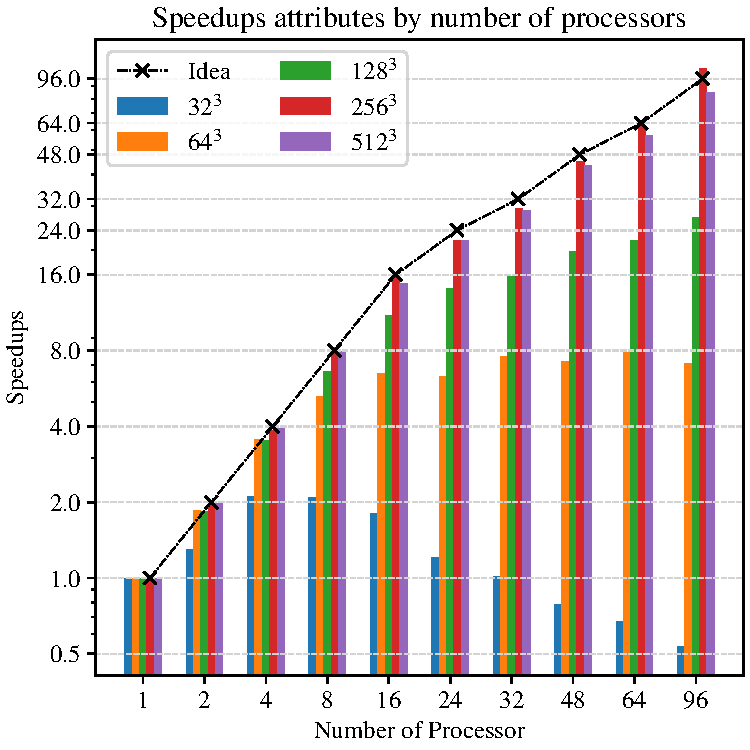
\includegraphics[width=0.45\textwidth]{figure/FIG_Benchmark_pure_mpi_3D.pdf}
    \label{FIG:Benchmark:Pure_MPI_Single_Node_3D}
  }
  \hfill
  \subfigure[Strong scaling on four node]
  {
    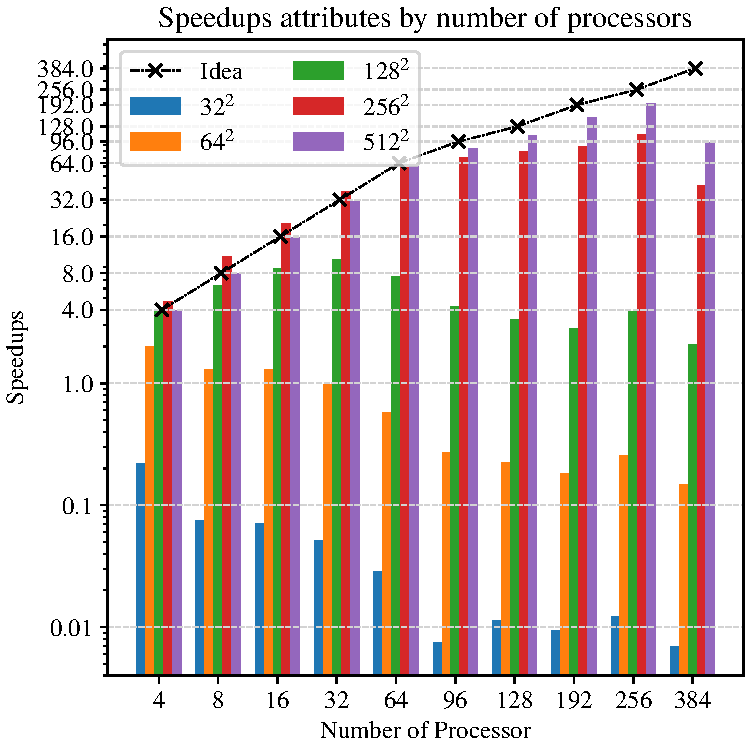
\includegraphics[width=0.45\textwidth]{figure/FIG_Benchmark_pure_mpi_3D_multi_nodes.pdf}
    \label{FIG:Benchmark:Pure_MPI_Multi_Node_3D}
  }
  \caption{
    Comparison of speedup ratios of strong scaling tests  pure MPI models on $4$ nodes of and $1$ node.
    The problem sizes are set to $32^3$, $64^3$, $128^3$, $256^3$ and $512^3$ and data type is \texttt{Double}.
  }
  \label{FIG:Benchmark:Pure_MPI_Node_3D}
\end{figure}

On the other hand, I specify the maximun scale of problem is $512^3$ rather than $1024^3$. 
This is because the pattern of accessing memories is $O(n^3)$ space complexity which leads more time consumption per epoch, 
although the problem has identical scale $1024^3 = 32768^2$. 
It also makes us harder to see a large superlinear speedup occurs comparing to 2D problems.
In this scenario, only the figure \ref{FIG:Benchmark:Pure_MPI_Multi_Node_3D} shows that the problem with scale $256^3$ has 
superlinear speedup on $8$, $16$ and $32$ CPUs due to the separated nodes has dependent CPU clock whic increase the rate of hitting cache.
\begin{figure}[htbp]
  \centering
  \subfigure[Single]{
    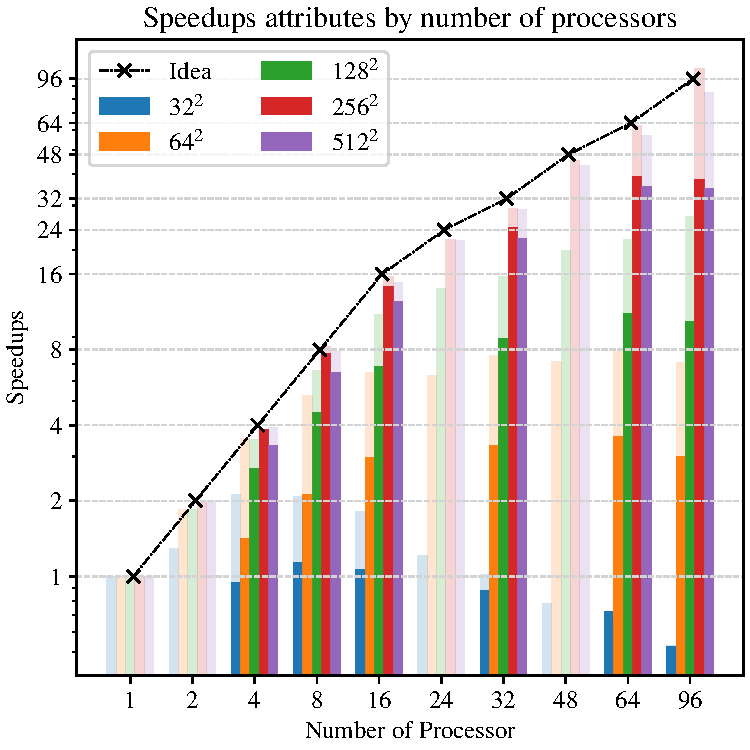
\includegraphics[width=0.38\textwidth]{figure/FIG_Benchmark_hybrid_0_single_nodes_3D.pdf}
    \label{FIG:Benchmark:FIG_Benchmark_hybrid_0_single_nodes_3D}
  }
  \hspace{0em} 
  \subfigure[Single]{
    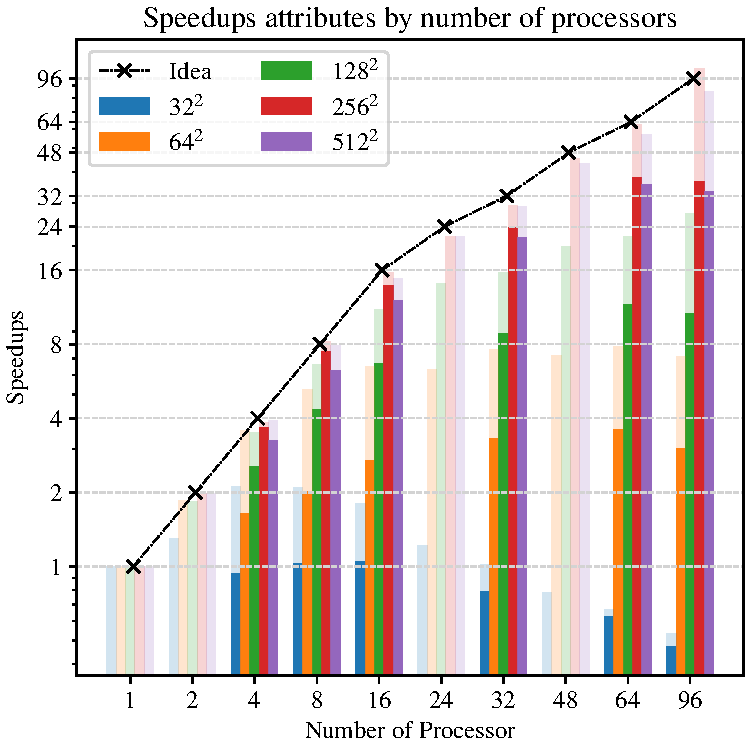
\includegraphics[width=0.38\textwidth]{figure/FIG_Benchmark_hybrid_1_single_nodes_3D.pdf}
    \label{FIG:Benchmark:FIG_Benchmark_hybrid_1_single_nodes_3D}
  }
  \hspace{0em} 
  \subfigure[caption]{
    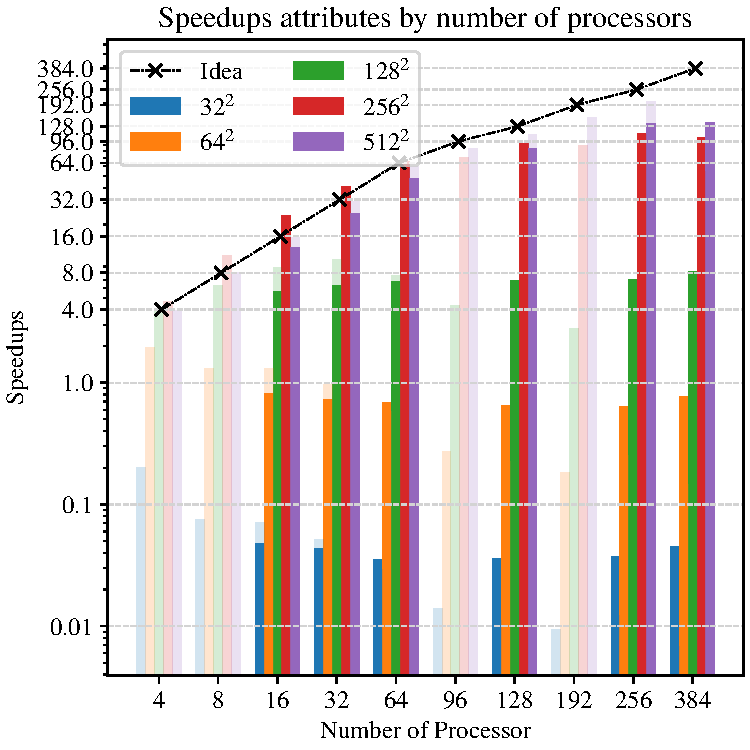
\includegraphics[width=0.38\textwidth]{figure/FIG_Benchmark_hybrid_0_multi_nodes_3D.pdf}
    \label{FIG:Benchmark:FIG_Benchmark_hybrid_0_multi_nodes_3D}
  }
  \hspace{0em} 
  \subfigure[caption]{
    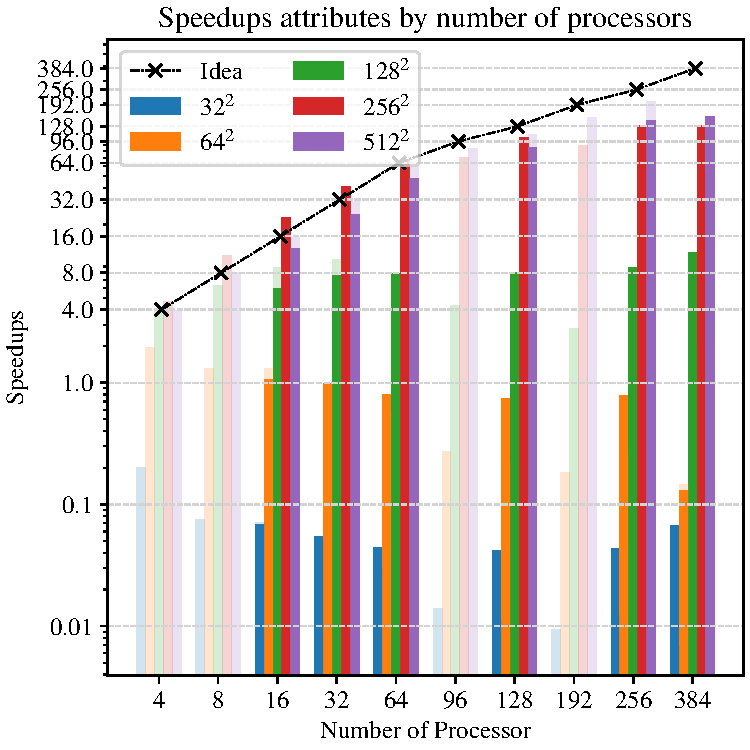
\includegraphics[width=0.38\textwidth]{figure/FIG_Benchmark_hybrid_1_multi_nodes_3D.pdf}
    \label{FIG:Benchmark:FIG_Benchmark_hybrid_1_multi_nodes_3D}
  }
  \caption{<caption>}
  \label{FIG:Benchmark:Hybrid_Single_Four_Node_3D}
\end{figure}

% \begin{wrapfigure}{r}{0.8\textwidth} 
%   \centering
%   \subfigure[Single]{
%     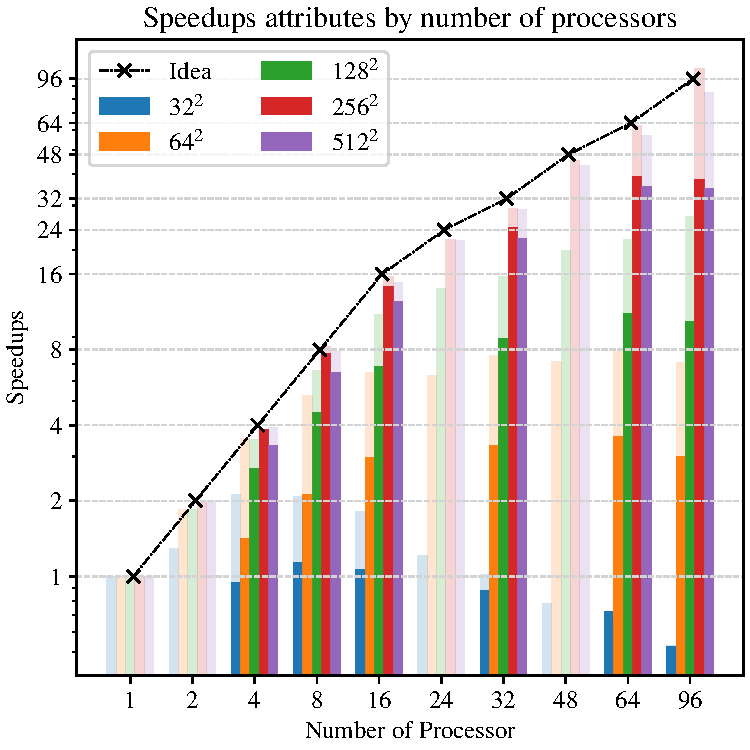
\includegraphics[width=0.35\textwidth]{figure/FIG_Benchmark_hybrid_0_single_nodes_3D.pdf}
%     \label{FIG:Benchmark:FIG_Benchmark_hybrid_0_single_nodes_3D}
%   }
%   \hspace{0em} 
%   \subfigure[Single]{
%     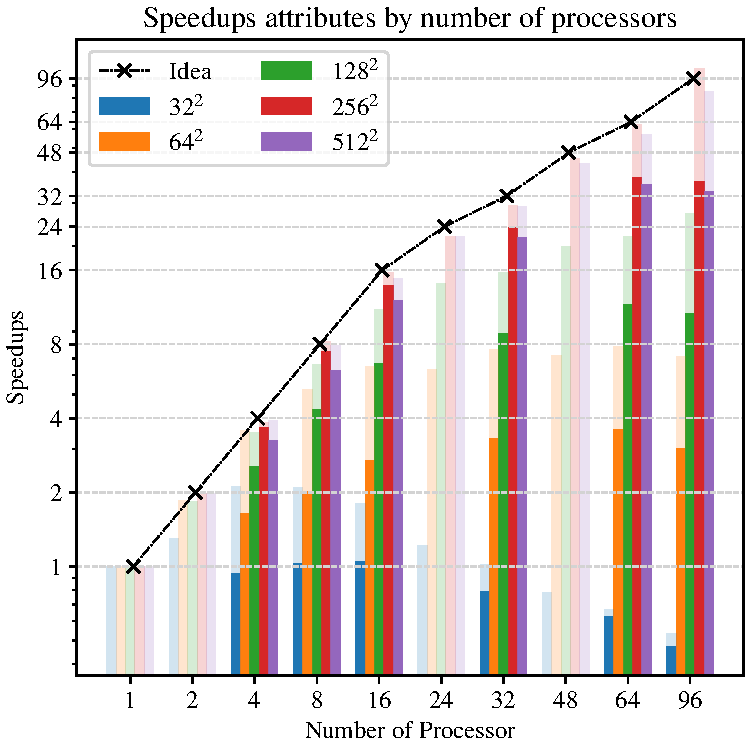
\includegraphics[width=0.35\textwidth]{figure/FIG_Benchmark_hybrid_1_single_nodes_3D.pdf}
%     \label{FIG:Benchmark:FIG_Benchmark_hybrid_1_single_nodes_3D}
%   }
%   \hspace{0em} 
%   \subfigure[caption]{
%     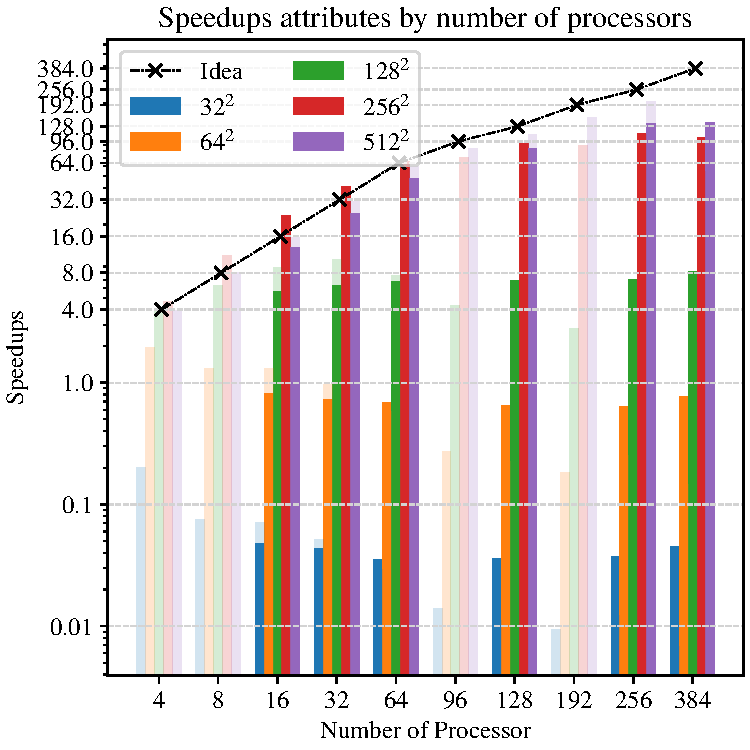
\includegraphics[width=0.35\textwidth]{figure/FIG_Benchmark_hybrid_0_multi_nodes_3D.pdf}
%     \label{FIG:Benchmark:FIG_Benchmark_hybrid_0_multi_nodes_3D}
%   }
%   \hspace{0em} 
%   \subfigure[caption]{
%     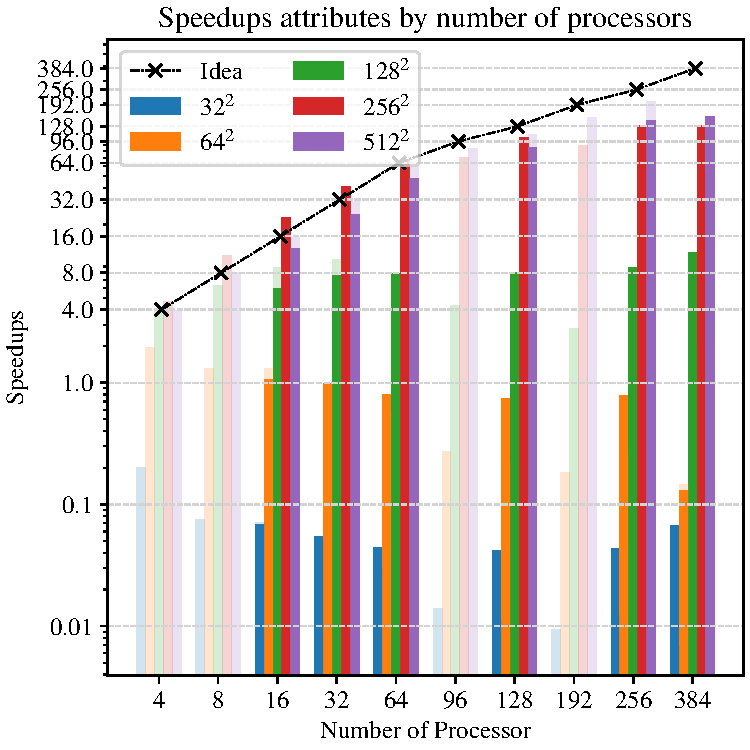
\includegraphics[width=0.35\textwidth]{figure/FIG_Benchmark_hybrid_1_multi_nodes_3D.pdf}
%     \label{FIG:Benchmark:FIG_Benchmark_hybrid_1_multi_nodes_3D}
%   }
%   \caption{<caption>}
%   \label{FIG:Benchmark:Hybrid_Single_Four_Node_3D}
% \end{wrapfigure}
The figure \ref{FIG:Benchmark:Hybrid_Single_Four_Node_3D} shows the details of hybrid parallel models on single and four nodes.
Overall, the figures \ref{FIG:Benchmark:FIG_Benchmark_hybrid_0_single_nodes_3D} and \ref{FIG:Benchmark:FIG_Benchmark_hybrid_1_single_nodes_3D}
show that both hybrid model have worse performance on single node. Even with the benefits of caching, the $256^3$ scale problem still 
a little bit loss on speedup on $4$, $8$ and $16$ CPUs.
However the figures \ref{FIG:Benchmark:FIG_Benchmark_hybrid_0_multi_nodes_3D} and \ref{FIG:Benchmark:FIG_Benchmark_hybrid_1_single_nodes_3D} 
shows completely different results.
On the multi-nodes test, overall, all hybrid models have better performance comparing to pure MPI parallelization.
Especially for the largest problem $512^3$ which the pure MPI scaling speedup ratio is $96$ under $384$ CPUs, the 
hybrid models gained approximately $130$ and $140$ speedups which is about $30\% ~ 40\%$ improvements.
Moreover, the problem with $256^3$ scale investigated on $8$ $16$ and $32$ CPUs reached superlinear speedup at the end,
which were making use of L3 cache and asynchronized CPU clock cycle.

As for the promotion gets from the cache and CPU asynchronization, we can discovered that the 2D problems got less benefits 
while the 3D problems got bigger.
This is the 3D problem relys more on the memory accessing, and the shared memory parallelization can do optimizations better than MPI.

\subsubsection{Weak Scaling}

The weak scaling results of 3 dimension problems are listed in the table \ref{TAB:Benchmark:Weak_3D_AllModels}.
For the single node scaling speedups, we could see that the pure MPI model has better performance over all problem scales 
and amount of resources.
However, for the multi-node tests, the hybrid models have approximately same or better performance than pue MPI model.
Especially for the non-overlapped hybrid model.


% pure_mpi 32 14.205280130981388 [9.07797386]
% pure_mpi 64 47.05604671282058 [30.1075974]
% pure_mpi 128 39.74555364101945 [25.42773957]

% hybrid_0 32 12.667882915956632 [8.09379942]
% hybrid_0 64 52.292330736249745 [33.45963735]
% hybrid_0 128 31.59871392899227 [20.21248921]

% hybrid_1 32 14.998693266535422 [9.58588224]
% hybrid_1 64 55.094846355099 [35.25368524]
% hybrid_1 128 31.416593371177605 [20.0959036]

\begin{table}[htbp]
  \caption{Weak Scaling of 3D Heat Equation}
  \label{TAB:Benchmark:Weak_3D_AllModels}
  \begin{minipage}{\columnwidth}
    \begin{center}
      \footnotesize % overleaf
      \begin{tabular}{>{\bfseries}p{2.5cm} p{1cm} p{1.5cm} p{1.5cm} p{1.5cm} p{1.5cm} p{1cm} p{1cm}}
        \toprule
        \multirow{2}{*}{Strategy} & \multirow{2}{*}{\bfseries Size} & \multicolumn{3}{c}{\bfseries  Number of CPUs}    & \multirow{2}{*}{\bfseries $f_p(\%)$}  & \multirow{2}{*}{\bfseries $f_p(\%)_{\text{Multi-node}}$}\\
                      &                      & \bfseries 8     & \bfseries 64        & \bfseries 64$_{\text{Multi-node}}$   &  &  &         \\
        \midrule
        Pure MPI      & \multirow{3}{*}{$32^3$}       & 5.243  & 26.405              &  9.078                     & 41.6 & 14.2 \\
        No Overlap    &                               & 2.124  & 13.386              &  8.094                     & 21.0 &  12.7\\
        With Overlap  &                               & 2.014  & 13.884              &  9.586                     & 21.8 & 39.7 \\
        \midrule
        Pure MPI      & \multirow{3}{*}{$64^3$}       & 7.937  & 32.034              &  30.106                    & 50.8 & 47.1 \\
        No Overlap    &                               & 5.393  & 20.007              &  33.460                    & 31.8 & 52.3 \\
        With Overlap  &                               & 5.200  & 19.558              &  35.254                    & 31.1 & 31.6 \\
        \midrule
        Pure MPI      & \multirow{3}{*}{$128^3$}      & 3.513  & 24.239              &  25.428                    & 38.0 & 39.7 \\
        No Overlap    &                               & 3.303  & 15.235              &  35.254                    & 24.1 & 55.1 \\
        With Overlap  &                               & 3.187  & 15.107              &  20.096                    & 23.9 & 31.4 \\
        \bottomrule
      \end{tabular}
    \end{center}
    % \bigskip
    % \footnotesize\emph{Source:} This is source 
  \end{minipage}
\end{table}

On the other hand, comparing the results from 2 dimension versions shown in table \ref{TAB:Benchmark:Weak_PURE_MPI} and \ref{TAB:Benchmark:Weak_PURE_MPI_Multi_Node}.
It is readily to determine that the weak scaling speedup of 3 dimension problems are worse than 2 dimensions.
Which means that the fraction of parallelizable parts in 3D problems are significantly lower than 2D version.


% \begin{wrapfigure}{r}{0.45\textwidth} 
%   \centering
%   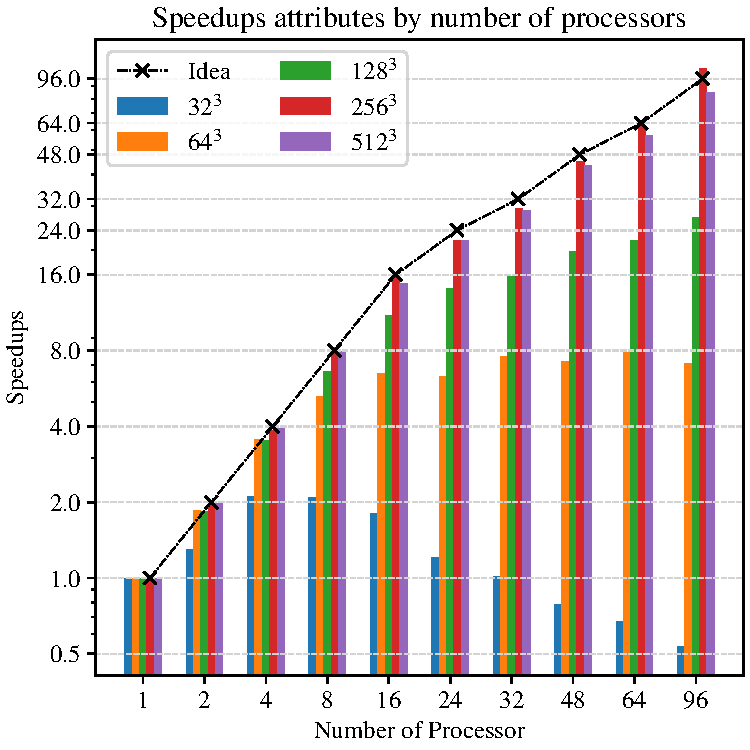
\includegraphics[width=0.5\textwidth]{figure/FIG_Benchmark_pure_mpi_3D.pdf}
%   \caption{
%     Comparison of speedup ratios of strong scaling tests of pure MPI parallelized program. 
%     % The investigated problem scales are the power of $2$, exponents ranging from $9$ to $15$.
%     % The number of CPUs are also set as power of $2$, with additional numbers $24$, $48$ and $96$ matched the topologies of CPU.
%   }
%   \label{FIG:Benchmark:PURE_MPI_3D}
% \end{wrapfigure}















\subsection{Comparison on Accuracy, with PINN}
Scalability is important for parallel computing to be effective, so as the quality of results.
In this section, the major comparison are about comparing the quality of numerical solutions of 
2D, 3D FDTD solvers and a state-of-art method PINN.


\subsubsection{Accuracy}
When we tried to represent numbers using arithmetic in binary, decimal or hexadecimal, truncation always affects the precision of every number, 
or so called as 
round-off-error.

\paragraph{Round-off Error}
In IEEE-754 \cite{IEEE_754} standards, a $32$-bit floating pointer number, single precision, obligatorily represented with $23$-bit mantissa, 
$8$-bit exponent and $1$-bit for sign. 
Where as $64$-bit floating number, double precision, also ubiquitous used, which has $11$-bit exponent and $52$-bit mantissa.
After almost three decades development, not only single and double precisions (float32, float64) are ubiquitously in use, 
also more formats such as fp4, fp8, and fp16 etc. Both of them follows the simple form of exponent $k$, sign $n$ and mantissa $N$. 
\cite{IEEE_754_p2_eq1}
\begin{equation*}
  2^{k+1-N}n
\end{equation*}
Round-off errors are a manifestation of the fact that on a digital computer, which is unavoidable in numerical computations.
In such case, the precision of the number depends on how many bytes are used to store single number. 
For instance, a float32 number provides $2^{-23} \approx 1.2\times10^{-7}$, and a double precision number gives $2^{-53} \approx 2.2\times10^{-16}$, 
such number is called machine $\epsilon$ which is the smallest number the machine can represent with given format.

In numerical methods I investigated, the FDTDs are conventionally using double precision number so that the programs can treat extreamly large and small 
numbers simultaneously in the same computation, without worring about the round-off errors.
However, as mentioned, fp32 and fp16 are also popular use in scientific computing, especially in machine learning training process. 
While the lasted training GPUs are integrated compute accelarate unit for low precision floating numbers. \cite{NVIDIA_HB200_PAPER}.

\paragraph{Floating-point Arithmetic}
The other type loss comes from the arithmetic operations on two numbers $x$, $y$. 
The standard model holds that 
\begin{equation}
  fl(x \:\text{op}\: y) = (x \: \text{op} \: y) (1+\delta), \:\:\: \left|\delta\right| < \epsilon
\end{equation}
where the $op$ stands for the four elementary operations: $+, -, \times, /$. \cite{Germund,NMSC,V1,P112}.




% \subsection{Finite Difference Methods}
% \subsubsection{Pure Message Passing Parallel}
% \subsubsection{Hybrid Parallel}


% \subsection{Physics Informed Neural Networks}
% \subsubsection{CUDA parallel}
% \subsubsection{Hybrid Parallel}


% \subsection{Visualization}


% \subsection{Comparison on Boundary Conditions}










% Table 
% lists the results 

% \begin{table}
%   \caption{Strong Scaling on Single Node of 2D Heat Equation}
%   \label{}
%   \begin{minipage}{\columnwidth}
%     \begin{center}
%       \begin{tabular}{lcccccc}
%         \toprule
%         Scale & $1024^2$ & $2048^2$ & $4096^2$  & $8192^2$  & $16384^2$ & $32768^2$\\
%         \midrule
%         2     & 1        & 1        &   1       & 1         & 1         & 1 \\
%         4     & 1        & 1        &   1       & 1         & 1         & 1 \\
%         8     & 1        & 1        &   1       & 1         & 1         & 1 \\
%         16     & 1        & 1        &   1       & 1         & 1         & 1 \\
%         32     & 1        & 1        &   1       & 1         & 1         & 1 \\
%         48     & 1        & 1        &   1       & 1         & 1         & 1 \\
%         64     & 1        & 1        &   1       & 1         & 1         & 1 \\
%         96     & 1        & 1        &   1       & 1         & 1         & 1 \\
%         \bottomrule
%       \end{tabular}
%     \end{center}
%     % \bigskip
%     % \footnotesize\emph{Source:} This is source 
%   \end{minipage}
% \end{table}
\section{Experiments}
\section{Conclusion}
\section{Acknowledgement}


% \bibliographystyle{ACM-Reference-Format}
% \bibliography{reference}

\printbibliography

\appendix

\end{document}